\documentclass[article]{jss}
%% need no \usepackage{Sweave.sty}

\usepackage{color}%
\definecolor{highlightBg}{rgb}{0.949019607843137,0.949019607843137,0.949019607843137}
\definecolor{highlightBorder}{rgb}{0,0,0}
\newenvironment{Hinput}%
{}%
{}%
\newenvironment{Houtput}%
{}%
{}%
\newsavebox{\highlightbox}%
\newenvironment{Hchunk}%
{%
\vspace{0.5em}\noindent\begin{lrbox}{\highlightbox}%
\begin{minipage}[b]{.9\textwidth}%
}%
{%
\end{minipage}%
\end{lrbox}%
\fcolorbox{highlightBorder}{highlightBg}{\usebox{\highlightbox}}%
\vspace{0.5em}}%


\usepackage{color}%
 
\newsavebox{\hlnormalsizeboxclosebrace}%
\newsavebox{\hlnormalsizeboxopenbrace}%
\newsavebox{\hlnormalsizeboxbackslash}%
\newsavebox{\hlnormalsizeboxlessthan}%
\newsavebox{\hlnormalsizeboxgreaterthan}%
\newsavebox{\hlnormalsizeboxdollar}%
\newsavebox{\hlnormalsizeboxunderscore}%
\newsavebox{\hlnormalsizeboxand}%
\newsavebox{\hlnormalsizeboxhash}%
\newsavebox{\hlnormalsizeboxat}%
\newsavebox{\hlnormalsizeboxpercent}% 
\newsavebox{\hlnormalsizeboxhat}%
\newsavebox{\hlnormalsizeboxsinglequote}%
\newsavebox{\hlnormalsizeboxbacktick}%

\setbox\hlnormalsizeboxopenbrace=\hbox{\begin{normalsize}\verb.{.\end{normalsize}}%
\setbox\hlnormalsizeboxclosebrace=\hbox{\begin{normalsize}\verb.}.\end{normalsize}}%
\setbox\hlnormalsizeboxlessthan=\hbox{\begin{normalsize}\verb.<.\end{normalsize}}%
\setbox\hlnormalsizeboxdollar=\hbox{\begin{normalsize}\verb.$.\end{normalsize}}%
\setbox\hlnormalsizeboxunderscore=\hbox{\begin{normalsize}\verb._.\end{normalsize}}%
\setbox\hlnormalsizeboxand=\hbox{\begin{normalsize}\verb.&.\end{normalsize}}%
\setbox\hlnormalsizeboxhash=\hbox{\begin{normalsize}\verb.#.\end{normalsize}}%
\setbox\hlnormalsizeboxat=\hbox{\begin{normalsize}\verb.@.\end{normalsize}}%
\setbox\hlnormalsizeboxbackslash=\hbox{\begin{normalsize}\verb.\.\end{normalsize}}%
\setbox\hlnormalsizeboxgreaterthan=\hbox{\begin{normalsize}\verb.>.\end{normalsize}}%
\setbox\hlnormalsizeboxpercent=\hbox{\begin{normalsize}\verb.%.\end{normalsize}}%
\setbox\hlnormalsizeboxhat=\hbox{\begin{normalsize}\verb.^.\end{normalsize}}%
\setbox\hlnormalsizeboxsinglequote=\hbox{\begin{normalsize}\verb.'.\end{normalsize}}%
\setbox\hlnormalsizeboxbacktick=\hbox{\begin{normalsize}\verb.`.\end{normalsize}}%
\setbox\hlnormalsizeboxhat=\hbox{\begin{normalsize}\verb.^.\end{normalsize}}%



\newsavebox{\hltinyboxclosebrace}%
\newsavebox{\hltinyboxopenbrace}%
\newsavebox{\hltinyboxbackslash}%
\newsavebox{\hltinyboxlessthan}%
\newsavebox{\hltinyboxgreaterthan}%
\newsavebox{\hltinyboxdollar}%
\newsavebox{\hltinyboxunderscore}%
\newsavebox{\hltinyboxand}%
\newsavebox{\hltinyboxhash}%
\newsavebox{\hltinyboxat}%
\newsavebox{\hltinyboxpercent}% 
\newsavebox{\hltinyboxhat}%
\newsavebox{\hltinyboxsinglequote}%
\newsavebox{\hltinyboxbacktick}%

\setbox\hltinyboxopenbrace=\hbox{\begin{tiny}\verb.{.\end{tiny}}%
\setbox\hltinyboxclosebrace=\hbox{\begin{tiny}\verb.}.\end{tiny}}%
\setbox\hltinyboxlessthan=\hbox{\begin{tiny}\verb.<.\end{tiny}}%
\setbox\hltinyboxdollar=\hbox{\begin{tiny}\verb.$.\end{tiny}}%
\setbox\hltinyboxunderscore=\hbox{\begin{tiny}\verb._.\end{tiny}}%
\setbox\hltinyboxand=\hbox{\begin{tiny}\verb.&.\end{tiny}}%
\setbox\hltinyboxhash=\hbox{\begin{tiny}\verb.#.\end{tiny}}%
\setbox\hltinyboxat=\hbox{\begin{tiny}\verb.@.\end{tiny}}%
\setbox\hltinyboxbackslash=\hbox{\begin{tiny}\verb.\.\end{tiny}}%
\setbox\hltinyboxgreaterthan=\hbox{\begin{tiny}\verb.>.\end{tiny}}%
\setbox\hltinyboxpercent=\hbox{\begin{tiny}\verb.%.\end{tiny}}%
\setbox\hltinyboxhat=\hbox{\begin{tiny}\verb.^.\end{tiny}}%
\setbox\hltinyboxsinglequote=\hbox{\begin{tiny}\verb.'.\end{tiny}}%
\setbox\hltinyboxbacktick=\hbox{\begin{tiny}\verb.`.\end{tiny}}%
\setbox\hltinyboxhat=\hbox{\begin{tiny}\verb.^.\end{tiny}}%



\newsavebox{\hlscriptsizeboxclosebrace}%
\newsavebox{\hlscriptsizeboxopenbrace}%
\newsavebox{\hlscriptsizeboxbackslash}%
\newsavebox{\hlscriptsizeboxlessthan}%
\newsavebox{\hlscriptsizeboxgreaterthan}%
\newsavebox{\hlscriptsizeboxdollar}%
\newsavebox{\hlscriptsizeboxunderscore}%
\newsavebox{\hlscriptsizeboxand}%
\newsavebox{\hlscriptsizeboxhash}%
\newsavebox{\hlscriptsizeboxat}%
\newsavebox{\hlscriptsizeboxpercent}% 
\newsavebox{\hlscriptsizeboxhat}%
\newsavebox{\hlscriptsizeboxsinglequote}%
\newsavebox{\hlscriptsizeboxbacktick}%

\setbox\hlscriptsizeboxopenbrace=\hbox{\begin{scriptsize}\verb.{.\end{scriptsize}}%
\setbox\hlscriptsizeboxclosebrace=\hbox{\begin{scriptsize}\verb.}.\end{scriptsize}}%
\setbox\hlscriptsizeboxlessthan=\hbox{\begin{scriptsize}\verb.<.\end{scriptsize}}%
\setbox\hlscriptsizeboxdollar=\hbox{\begin{scriptsize}\verb.$.\end{scriptsize}}%
\setbox\hlscriptsizeboxunderscore=\hbox{\begin{scriptsize}\verb._.\end{scriptsize}}%
\setbox\hlscriptsizeboxand=\hbox{\begin{scriptsize}\verb.&.\end{scriptsize}}%
\setbox\hlscriptsizeboxhash=\hbox{\begin{scriptsize}\verb.#.\end{scriptsize}}%
\setbox\hlscriptsizeboxat=\hbox{\begin{scriptsize}\verb.@.\end{scriptsize}}%
\setbox\hlscriptsizeboxbackslash=\hbox{\begin{scriptsize}\verb.\.\end{scriptsize}}%
\setbox\hlscriptsizeboxgreaterthan=\hbox{\begin{scriptsize}\verb.>.\end{scriptsize}}%
\setbox\hlscriptsizeboxpercent=\hbox{\begin{scriptsize}\verb.%.\end{scriptsize}}%
\setbox\hlscriptsizeboxhat=\hbox{\begin{scriptsize}\verb.^.\end{scriptsize}}%
\setbox\hlscriptsizeboxsinglequote=\hbox{\begin{scriptsize}\verb.'.\end{scriptsize}}%
\setbox\hlscriptsizeboxbacktick=\hbox{\begin{scriptsize}\verb.`.\end{scriptsize}}%
\setbox\hlscriptsizeboxhat=\hbox{\begin{scriptsize}\verb.^.\end{scriptsize}}%



\newsavebox{\hlfootnotesizeboxclosebrace}%
\newsavebox{\hlfootnotesizeboxopenbrace}%
\newsavebox{\hlfootnotesizeboxbackslash}%
\newsavebox{\hlfootnotesizeboxlessthan}%
\newsavebox{\hlfootnotesizeboxgreaterthan}%
\newsavebox{\hlfootnotesizeboxdollar}%
\newsavebox{\hlfootnotesizeboxunderscore}%
\newsavebox{\hlfootnotesizeboxand}%
\newsavebox{\hlfootnotesizeboxhash}%
\newsavebox{\hlfootnotesizeboxat}%
\newsavebox{\hlfootnotesizeboxpercent}% 
\newsavebox{\hlfootnotesizeboxhat}%
\newsavebox{\hlfootnotesizeboxsinglequote}%
\newsavebox{\hlfootnotesizeboxbacktick}%

\setbox\hlfootnotesizeboxopenbrace=\hbox{\begin{footnotesize}\verb.{.\end{footnotesize}}%
\setbox\hlfootnotesizeboxclosebrace=\hbox{\begin{footnotesize}\verb.}.\end{footnotesize}}%
\setbox\hlfootnotesizeboxlessthan=\hbox{\begin{footnotesize}\verb.<.\end{footnotesize}}%
\setbox\hlfootnotesizeboxdollar=\hbox{\begin{footnotesize}\verb.$.\end{footnotesize}}%
\setbox\hlfootnotesizeboxunderscore=\hbox{\begin{footnotesize}\verb._.\end{footnotesize}}%
\setbox\hlfootnotesizeboxand=\hbox{\begin{footnotesize}\verb.&.\end{footnotesize}}%
\setbox\hlfootnotesizeboxhash=\hbox{\begin{footnotesize}\verb.#.\end{footnotesize}}%
\setbox\hlfootnotesizeboxat=\hbox{\begin{footnotesize}\verb.@.\end{footnotesize}}%
\setbox\hlfootnotesizeboxbackslash=\hbox{\begin{footnotesize}\verb.\.\end{footnotesize}}%
\setbox\hlfootnotesizeboxgreaterthan=\hbox{\begin{footnotesize}\verb.>.\end{footnotesize}}%
\setbox\hlfootnotesizeboxpercent=\hbox{\begin{footnotesize}\verb.%.\end{footnotesize}}%
\setbox\hlfootnotesizeboxhat=\hbox{\begin{footnotesize}\verb.^.\end{footnotesize}}%
\setbox\hlfootnotesizeboxsinglequote=\hbox{\begin{footnotesize}\verb.'.\end{footnotesize}}%
\setbox\hlfootnotesizeboxbacktick=\hbox{\begin{footnotesize}\verb.`.\end{footnotesize}}%
\setbox\hlfootnotesizeboxhat=\hbox{\begin{footnotesize}\verb.^.\end{footnotesize}}%



\newsavebox{\hlsmallboxclosebrace}%
\newsavebox{\hlsmallboxopenbrace}%
\newsavebox{\hlsmallboxbackslash}%
\newsavebox{\hlsmallboxlessthan}%
\newsavebox{\hlsmallboxgreaterthan}%
\newsavebox{\hlsmallboxdollar}%
\newsavebox{\hlsmallboxunderscore}%
\newsavebox{\hlsmallboxand}%
\newsavebox{\hlsmallboxhash}%
\newsavebox{\hlsmallboxat}%
\newsavebox{\hlsmallboxpercent}% 
\newsavebox{\hlsmallboxhat}%
\newsavebox{\hlsmallboxsinglequote}%
\newsavebox{\hlsmallboxbacktick}%

\setbox\hlsmallboxopenbrace=\hbox{\begin{small}\verb.{.\end{small}}%
\setbox\hlsmallboxclosebrace=\hbox{\begin{small}\verb.}.\end{small}}%
\setbox\hlsmallboxlessthan=\hbox{\begin{small}\verb.<.\end{small}}%
\setbox\hlsmallboxdollar=\hbox{\begin{small}\verb.$.\end{small}}%
\setbox\hlsmallboxunderscore=\hbox{\begin{small}\verb._.\end{small}}%
\setbox\hlsmallboxand=\hbox{\begin{small}\verb.&.\end{small}}%
\setbox\hlsmallboxhash=\hbox{\begin{small}\verb.#.\end{small}}%
\setbox\hlsmallboxat=\hbox{\begin{small}\verb.@.\end{small}}%
\setbox\hlsmallboxbackslash=\hbox{\begin{small}\verb.\.\end{small}}%
\setbox\hlsmallboxgreaterthan=\hbox{\begin{small}\verb.>.\end{small}}%
\setbox\hlsmallboxpercent=\hbox{\begin{small}\verb.%.\end{small}}%
\setbox\hlsmallboxhat=\hbox{\begin{small}\verb.^.\end{small}}%
\setbox\hlsmallboxsinglequote=\hbox{\begin{small}\verb.'.\end{small}}%
\setbox\hlsmallboxbacktick=\hbox{\begin{small}\verb.`.\end{small}}%
\setbox\hlsmallboxhat=\hbox{\begin{small}\verb.^.\end{small}}%



\newsavebox{\hllargeboxclosebrace}%
\newsavebox{\hllargeboxopenbrace}%
\newsavebox{\hllargeboxbackslash}%
\newsavebox{\hllargeboxlessthan}%
\newsavebox{\hllargeboxgreaterthan}%
\newsavebox{\hllargeboxdollar}%
\newsavebox{\hllargeboxunderscore}%
\newsavebox{\hllargeboxand}%
\newsavebox{\hllargeboxhash}%
\newsavebox{\hllargeboxat}%
\newsavebox{\hllargeboxpercent}% 
\newsavebox{\hllargeboxhat}%
\newsavebox{\hllargeboxsinglequote}%
\newsavebox{\hllargeboxbacktick}%

\setbox\hllargeboxopenbrace=\hbox{\begin{large}\verb.{.\end{large}}%
\setbox\hllargeboxclosebrace=\hbox{\begin{large}\verb.}.\end{large}}%
\setbox\hllargeboxlessthan=\hbox{\begin{large}\verb.<.\end{large}}%
\setbox\hllargeboxdollar=\hbox{\begin{large}\verb.$.\end{large}}%
\setbox\hllargeboxunderscore=\hbox{\begin{large}\verb._.\end{large}}%
\setbox\hllargeboxand=\hbox{\begin{large}\verb.&.\end{large}}%
\setbox\hllargeboxhash=\hbox{\begin{large}\verb.#.\end{large}}%
\setbox\hllargeboxat=\hbox{\begin{large}\verb.@.\end{large}}%
\setbox\hllargeboxbackslash=\hbox{\begin{large}\verb.\.\end{large}}%
\setbox\hllargeboxgreaterthan=\hbox{\begin{large}\verb.>.\end{large}}%
\setbox\hllargeboxpercent=\hbox{\begin{large}\verb.%.\end{large}}%
\setbox\hllargeboxhat=\hbox{\begin{large}\verb.^.\end{large}}%
\setbox\hllargeboxsinglequote=\hbox{\begin{large}\verb.'.\end{large}}%
\setbox\hllargeboxbacktick=\hbox{\begin{large}\verb.`.\end{large}}%
\setbox\hllargeboxhat=\hbox{\begin{large}\verb.^.\end{large}}%



\newsavebox{\hlLargeboxclosebrace}%
\newsavebox{\hlLargeboxopenbrace}%
\newsavebox{\hlLargeboxbackslash}%
\newsavebox{\hlLargeboxlessthan}%
\newsavebox{\hlLargeboxgreaterthan}%
\newsavebox{\hlLargeboxdollar}%
\newsavebox{\hlLargeboxunderscore}%
\newsavebox{\hlLargeboxand}%
\newsavebox{\hlLargeboxhash}%
\newsavebox{\hlLargeboxat}%
\newsavebox{\hlLargeboxpercent}% 
\newsavebox{\hlLargeboxhat}%
\newsavebox{\hlLargeboxsinglequote}%
\newsavebox{\hlLargeboxbacktick}%

\setbox\hlLargeboxopenbrace=\hbox{\begin{Large}\verb.{.\end{Large}}%
\setbox\hlLargeboxclosebrace=\hbox{\begin{Large}\verb.}.\end{Large}}%
\setbox\hlLargeboxlessthan=\hbox{\begin{Large}\verb.<.\end{Large}}%
\setbox\hlLargeboxdollar=\hbox{\begin{Large}\verb.$.\end{Large}}%
\setbox\hlLargeboxunderscore=\hbox{\begin{Large}\verb._.\end{Large}}%
\setbox\hlLargeboxand=\hbox{\begin{Large}\verb.&.\end{Large}}%
\setbox\hlLargeboxhash=\hbox{\begin{Large}\verb.#.\end{Large}}%
\setbox\hlLargeboxat=\hbox{\begin{Large}\verb.@.\end{Large}}%
\setbox\hlLargeboxbackslash=\hbox{\begin{Large}\verb.\.\end{Large}}%
\setbox\hlLargeboxgreaterthan=\hbox{\begin{Large}\verb.>.\end{Large}}%
\setbox\hlLargeboxpercent=\hbox{\begin{Large}\verb.%.\end{Large}}%
\setbox\hlLargeboxhat=\hbox{\begin{Large}\verb.^.\end{Large}}%
\setbox\hlLargeboxsinglequote=\hbox{\begin{Large}\verb.'.\end{Large}}%
\setbox\hlLargeboxbacktick=\hbox{\begin{Large}\verb.`.\end{Large}}%
\setbox\hlLargeboxhat=\hbox{\begin{Large}\verb.^.\end{Large}}%



\newsavebox{\hlLARGEboxclosebrace}%
\newsavebox{\hlLARGEboxopenbrace}%
\newsavebox{\hlLARGEboxbackslash}%
\newsavebox{\hlLARGEboxlessthan}%
\newsavebox{\hlLARGEboxgreaterthan}%
\newsavebox{\hlLARGEboxdollar}%
\newsavebox{\hlLARGEboxunderscore}%
\newsavebox{\hlLARGEboxand}%
\newsavebox{\hlLARGEboxhash}%
\newsavebox{\hlLARGEboxat}%
\newsavebox{\hlLARGEboxpercent}% 
\newsavebox{\hlLARGEboxhat}%
\newsavebox{\hlLARGEboxsinglequote}%
\newsavebox{\hlLARGEboxbacktick}%

\setbox\hlLARGEboxopenbrace=\hbox{\begin{LARGE}\verb.{.\end{LARGE}}%
\setbox\hlLARGEboxclosebrace=\hbox{\begin{LARGE}\verb.}.\end{LARGE}}%
\setbox\hlLARGEboxlessthan=\hbox{\begin{LARGE}\verb.<.\end{LARGE}}%
\setbox\hlLARGEboxdollar=\hbox{\begin{LARGE}\verb.$.\end{LARGE}}%
\setbox\hlLARGEboxunderscore=\hbox{\begin{LARGE}\verb._.\end{LARGE}}%
\setbox\hlLARGEboxand=\hbox{\begin{LARGE}\verb.&.\end{LARGE}}%
\setbox\hlLARGEboxhash=\hbox{\begin{LARGE}\verb.#.\end{LARGE}}%
\setbox\hlLARGEboxat=\hbox{\begin{LARGE}\verb.@.\end{LARGE}}%
\setbox\hlLARGEboxbackslash=\hbox{\begin{LARGE}\verb.\.\end{LARGE}}%
\setbox\hlLARGEboxgreaterthan=\hbox{\begin{LARGE}\verb.>.\end{LARGE}}%
\setbox\hlLARGEboxpercent=\hbox{\begin{LARGE}\verb.%.\end{LARGE}}%
\setbox\hlLARGEboxhat=\hbox{\begin{LARGE}\verb.^.\end{LARGE}}%
\setbox\hlLARGEboxsinglequote=\hbox{\begin{LARGE}\verb.'.\end{LARGE}}%
\setbox\hlLARGEboxbacktick=\hbox{\begin{LARGE}\verb.`.\end{LARGE}}%
\setbox\hlLARGEboxhat=\hbox{\begin{LARGE}\verb.^.\end{LARGE}}%



\newsavebox{\hlhugeboxclosebrace}%
\newsavebox{\hlhugeboxopenbrace}%
\newsavebox{\hlhugeboxbackslash}%
\newsavebox{\hlhugeboxlessthan}%
\newsavebox{\hlhugeboxgreaterthan}%
\newsavebox{\hlhugeboxdollar}%
\newsavebox{\hlhugeboxunderscore}%
\newsavebox{\hlhugeboxand}%
\newsavebox{\hlhugeboxhash}%
\newsavebox{\hlhugeboxat}%
\newsavebox{\hlhugeboxpercent}% 
\newsavebox{\hlhugeboxhat}%
\newsavebox{\hlhugeboxsinglequote}%
\newsavebox{\hlhugeboxbacktick}%

\setbox\hlhugeboxopenbrace=\hbox{\begin{huge}\verb.{.\end{huge}}%
\setbox\hlhugeboxclosebrace=\hbox{\begin{huge}\verb.}.\end{huge}}%
\setbox\hlhugeboxlessthan=\hbox{\begin{huge}\verb.<.\end{huge}}%
\setbox\hlhugeboxdollar=\hbox{\begin{huge}\verb.$.\end{huge}}%
\setbox\hlhugeboxunderscore=\hbox{\begin{huge}\verb._.\end{huge}}%
\setbox\hlhugeboxand=\hbox{\begin{huge}\verb.&.\end{huge}}%
\setbox\hlhugeboxhash=\hbox{\begin{huge}\verb.#.\end{huge}}%
\setbox\hlhugeboxat=\hbox{\begin{huge}\verb.@.\end{huge}}%
\setbox\hlhugeboxbackslash=\hbox{\begin{huge}\verb.\.\end{huge}}%
\setbox\hlhugeboxgreaterthan=\hbox{\begin{huge}\verb.>.\end{huge}}%
\setbox\hlhugeboxpercent=\hbox{\begin{huge}\verb.%.\end{huge}}%
\setbox\hlhugeboxhat=\hbox{\begin{huge}\verb.^.\end{huge}}%
\setbox\hlhugeboxsinglequote=\hbox{\begin{huge}\verb.'.\end{huge}}%
\setbox\hlhugeboxbacktick=\hbox{\begin{huge}\verb.`.\end{huge}}%
\setbox\hlhugeboxhat=\hbox{\begin{huge}\verb.^.\end{huge}}%



\newsavebox{\hlHugeboxclosebrace}%
\newsavebox{\hlHugeboxopenbrace}%
\newsavebox{\hlHugeboxbackslash}%
\newsavebox{\hlHugeboxlessthan}%
\newsavebox{\hlHugeboxgreaterthan}%
\newsavebox{\hlHugeboxdollar}%
\newsavebox{\hlHugeboxunderscore}%
\newsavebox{\hlHugeboxand}%
\newsavebox{\hlHugeboxhash}%
\newsavebox{\hlHugeboxat}%
\newsavebox{\hlHugeboxpercent}% 
\newsavebox{\hlHugeboxhat}%
\newsavebox{\hlHugeboxsinglequote}%
\newsavebox{\hlHugeboxbacktick}%

\setbox\hlHugeboxopenbrace=\hbox{\begin{Huge}\verb.{.\end{Huge}}%
\setbox\hlHugeboxclosebrace=\hbox{\begin{Huge}\verb.}.\end{Huge}}%
\setbox\hlHugeboxlessthan=\hbox{\begin{Huge}\verb.<.\end{Huge}}%
\setbox\hlHugeboxdollar=\hbox{\begin{Huge}\verb.$.\end{Huge}}%
\setbox\hlHugeboxunderscore=\hbox{\begin{Huge}\verb._.\end{Huge}}%
\setbox\hlHugeboxand=\hbox{\begin{Huge}\verb.&.\end{Huge}}%
\setbox\hlHugeboxhash=\hbox{\begin{Huge}\verb.#.\end{Huge}}%
\setbox\hlHugeboxat=\hbox{\begin{Huge}\verb.@.\end{Huge}}%
\setbox\hlHugeboxbackslash=\hbox{\begin{Huge}\verb.\.\end{Huge}}%
\setbox\hlHugeboxgreaterthan=\hbox{\begin{Huge}\verb.>.\end{Huge}}%
\setbox\hlHugeboxpercent=\hbox{\begin{Huge}\verb.%.\end{Huge}}%
\setbox\hlHugeboxhat=\hbox{\begin{Huge}\verb.^.\end{Huge}}%
\setbox\hlHugeboxsinglequote=\hbox{\begin{Huge}\verb.'.\end{Huge}}%
\setbox\hlHugeboxbacktick=\hbox{\begin{Huge}\verb.`.\end{Huge}}%
\setbox\hlHugeboxhat=\hbox{\begin{Huge}\verb.^.\end{Huge}}%
 

\def\urltilda{\kern -.15em\lower .7ex\hbox{\~{}}\kern .04em}%

\newcommand{\hlstd}[1]{\textcolor[rgb]{0,0,0}{#1}}%
\newcommand{\hlnum}[1]{\textcolor[rgb]{0.16,0.16,1}{#1}}
\newcommand{\hlesc}[1]{\textcolor[rgb]{1,0,1}{#1}}
\newcommand{\hlstr}[1]{\textcolor[rgb]{1,0,0}{#1}}
\newcommand{\hldstr}[1]{\textcolor[rgb]{0.51,0.51,0}{#1}}
\newcommand{\hlslc}[1]{\textcolor[rgb]{0.51,0.51,0.51}{\it{#1}}}
\newcommand{\hlcom}[1]{\textcolor[rgb]{0.51,0.51,0.51}{\it{#1}}}
\newcommand{\hldir}[1]{\textcolor[rgb]{0,0.51,0}{#1}}
\newcommand{\hlsym}[1]{\textcolor[rgb]{0,0,0}{#1}}
% \newcommand{\hlline}[1]{\textcolor[rgb]{0.33,0.33,0.33}{#1}}
\newcommand{\hlkwa}[1]{\textcolor[rgb]{0,0,0}{\bf{#1}}}
\newcommand{\hlkwb}[1]{\textcolor[rgb]{0.51,0,0}{#1}}
\newcommand{\hlkwc}[1]{\textcolor[rgb]{0,0,0}{\bf{#1}}}
\newcommand{\hlkwd}[1]{\textcolor[rgb]{0,0,0.51}{#1}}

\newcommand{\hlnumber}[1]{\textcolor[rgb]{0.0823529411764706,0.0784313725490196,0.709803921568627}{#1}}%
\newcommand{\hlfunctioncall}[1]{\textcolor[rgb]{1,0,0}{#1}}%
\newcommand{\hlstring}[1]{\textcolor[rgb]{0.6,0.6,1}{#1}}%
\newcommand{\hlkeyword}[1]{\textcolor[rgb]{0,0,0}{#1}}%
\newcommand{\hlargument}[1]{\textcolor[rgb]{0.694117647058824,0.247058823529412,0.0196078431372549}{#1}}%
\newcommand{\hlcomment}[1]{\textcolor[rgb]{0.8,0.8,0.8}{#1}}%
\newcommand{\hlroxygencomment}[1]{\textcolor[rgb]{0,0.592156862745098,1}{#1}}%
\newcommand{\hlformalargs}[1]{\textcolor[rgb]{0.0705882352941176,0.713725490196078,0.0705882352941176}{#1}}%
\newcommand{\hleqformalargs}[1]{\textcolor[rgb]{0.0705882352941176,0.713725490196078,0.0705882352941176}{#1}}%
\newcommand{\hlassignement}[1]{\textcolor[rgb]{0.215686274509804,0.215686274509804,0.384313725490196}{#1}}%
\newcommand{\hlpackage}[1]{\textcolor[rgb]{0.588235294117647,0.713725490196078,0.145098039215686}{#1}}%
\newcommand{\hlslot}[1]{\textit{#1}}%
\newcommand{\hlsymbol}[1]{\textcolor[rgb]{0,0,0}{#1}}%
\newcommand{\hlprompt}[1]{\textcolor[rgb]{0,0,0}{#1}}%
\newcommand{\hlline}[1]{\textcolor[rgb]{0.501960784313725,0.501960784313725,0.501960784313725}{#1}}%
\usepackage[utf8]{inputenc}
\usepackage{amsmath}

%%%%%%%%%%%%%%%%%%%%%%%%%%%%%%
%% declarations for jss.cls %%%%%%%%%%%%%%%%%%%%%%%%%%%%%%%%%%%%%%%%%%
%%%%%%%%%%%%%%%%%%%%%%%%%%%%%%

%% almost as usual
\author{Stefan Siegert\\University of Exeter}
\title{Verification Functions for Ensemble Forecasts Implemented in the \proglang{R} package \pkg{SpecsVerification}}

%% for pretty printing and a nice hypersummary also set:
\Plainauthor{Stefan Siegert} %% comma-separated
\Plaintitle{SpecsVerification: New R Functions for Verification of Ensemble Forecasts}
\Shorttitle{\pkg{SpecsVerification}: R Functions for Ensemble Verification} %% a short title (if necessary)

%% an abstract and keywords
\Abstract{

}
\Keywords{keywords, comma-separated, not capitalized, \proglang{Java}}
\Plainkeywords{keywords, comma-separated, not capitalized, Java} %% without formatting
%% at least one keyword must be supplied

%% publication information
%% NOTE: Typically, this can be left commented and will be filled out by the technical editor
%% \Volume{50}
%% \Issue{9}
%% \Month{June}
%% \Year{2012}
%% \Submitdate{2012-06-04}
%% \Acceptdate{2012-06-04}

%% The address of (at least) one author should be given
%% in the following format:
\Address{
  Stefan Siegert\\
  Exeter Climate Systems\\
  College for Engineering, Mathematics, and Physical Sciences\\
  University of Exeter\\
  Exeter, EX4 4QF, United Kingdom\\
  E-mail: \email{Stefan.Siegert@exeter.ac.uk}\\
  URL: \url{http://emps.exeter.ac.uk/mathematics/staff/ss610}
}

%% for those who use Sweave please include the following line (with % symbols):


%% end of declarations %%%%%%%%%%%%%%%%%%%%%%%%%%%%%%%%%%%%%%%%%%%%%%%


% initialise sweave


% initialise R session


\begin{document}



%% Note that you should use the \pkg{}, \proglang{} and \code{} commands.

% \section[About Java]{About \proglang{Java}}
%% Note: If there is markup in \(sub)section, then it has to be escape as above.


\section{Introduction}

{\bf SPECS}

{\bf Ensemble forecasting general}

deterministic, probabilistic, ensemble


{\bf Forecast verification general}
a posteriori comparison of forecasts with their verifying observations;
ensembles can be verified by taking the ensemble mean as a deterministic forecast; deriving a probability distribution and use a proper score; here: evaluate the raw ensemble

{\bf Finite size effect in ensemble verification}
Everything else being equal, larger ensembles yield better scores than smaller ensembles.


\begin{Hchunk}
\begin{normalsize}
\begin{Hinput}

\ttfamily\noindent
\hlprompt{{\ }}\hlfunctioncall{data}\hlkeyword{(}\hlsymbol{eurotempforecast}\hlkeyword{)}\mbox{}
\normalfont

\end{Hinput}


\begin{Hinput}

\ttfamily\noindent
\hlprompt{{\ }}\hlsymbol{ens}{\ }\hlassignement{\usebox{\hlnormalsizeboxlessthan}-}{\ }\hlsymbol{ens}\hlkeyword{[}\hlkeyword{,}{\ }\hlnumber{1}\hlkeyword{:}\hlnumber{8}\hlkeyword{]}\mbox{}
\normalfont

\end{Hinput}


\begin{Hinput}

\ttfamily\noindent
\hlprompt{{\ }}\hlsymbol{ens.bin}{\ }\hlassignement{\usebox{\hlnormalsizeboxlessthan}-}{\ }\hlsymbol{ens.bin}\hlkeyword{[}\hlkeyword{,}{\ }\hlnumber{1}\hlkeyword{:}\hlnumber{8}\hlkeyword{]}\mbox{}
\normalfont

\end{Hinput}


\begin{Hinput}

\ttfamily\noindent
\hlprompt{{\ }}\hlsymbol{ens.cat}{\ }\hlassignement{\usebox{\hlnormalsizeboxlessthan}-}{\ }\hlsymbol{ens.cat}\hlkeyword{[}\hlkeyword{,}{\ }\hlnumber{1}\hlkeyword{:}\hlnumber{8}\hlkeyword{]}\mbox{}
\normalfont

\end{Hinput}


\begin{Hinput}

\ttfamily\noindent
\hlprompt{{\ }}\hlsymbol{yrs}{\ }\hlassignement{\usebox{\hlnormalsizeboxlessthan}-}{\ }\hlfunctioncall{as.numeric}\hlkeyword{(}\hlfunctioncall{names}\hlkeyword{(}\hlsymbol{obs}\hlkeyword{)}\hlkeyword{)}\mbox{}
\normalfont

\end{Hinput}


\begin{Hinput}

\ttfamily\noindent
\hlprompt{{\ }}\hlsymbol{N}{\ }{\ }{\ }\hlassignement{\usebox{\hlnormalsizeboxlessthan}-}{\ }\hlfunctioncall{length}\hlkeyword{(}\hlsymbol{obs}\hlkeyword{)}\mbox{}
\normalfont

\end{Hinput}


\end{normalsize}
\end{Hchunk}



\begin{figure}
\begin{center}
%
\begin{Hchunk}
\begin{normalsize}
\begin{Hinput}

\ttfamily\noindent
\hlprompt{{\ }}\hlfunctioncall{par}\hlkeyword{(}\hlargument{las}\hlargument{=}\hlnumber{1}\hlkeyword{,}{\ }\hlargument{cex}\hlargument{=}\hlnumber{0.7}\hlkeyword{,}{\ }\hlargument{mgp}\hlargument{=}\hlfunctioncall{c}\hlkeyword{(}\hlnumber{3}\hlkeyword{,}{\ }\hlnumber{1}\hlkeyword{,}{\ }\hlnumber{0}\hlkeyword{)}\hlkeyword{,}{\ }\hlargument{mar}\hlargument{=}\hlfunctioncall{c}\hlkeyword{(}\hlnumber{2}\hlkeyword{,}\hlnumber{4}\hlkeyword{,}\hlnumber{1}\hlkeyword{,}\hlnumber{1}\hlkeyword{)}\hlkeyword{)}\mbox{}
\normalfont

\end{Hinput}


\begin{Hinput}

\ttfamily\noindent
\hlprompt{{\ }}\hlfunctioncall{plot}\hlkeyword{(}\hlnumber{NA}\hlkeyword{,}{\ }\hlargument{type}\hlargument{=}\hlstring{\usebox{\hlnormalsizeboxsinglequote}n\usebox{\hlnormalsizeboxsinglequote}}\hlkeyword{,}{\ }\hlargument{xlim}\hlargument{=}\hlfunctioncall{range}\hlkeyword{(}\hlsymbol{yrs}\hlkeyword{)}\hlkeyword{,}{\ }\hlargument{ylim}\hlargument{=}\hlfunctioncall{range}\hlkeyword{(}\hlfunctioncall{c}\hlkeyword{(}\hlsymbol{obs}\hlkeyword{,}{\ }\hlsymbol{ens}\hlkeyword{)}\hlkeyword{)}\hlkeyword{,}\hspace*{\fill}\\
\hlstd{}\hlprompt{{\ }}{\ }{\ }{\ }{\ }{\ }\hlargument{xlab}\hlargument{=}\hlstring{"{}"{}}\hlkeyword{,}{\ }\hlargument{ylab}\hlargument{=}\hlstring{"{}temp{\ }[C]"{}}\hlkeyword{)}\mbox{}
\normalfont

\end{Hinput}


\begin{Hinput}

\ttfamily\noindent
\hlprompt{{\ }}\hlkeyword{for}{\ }\hlkeyword{(}\hlsymbol{i}{\ }\hlkeyword{in}{\ }\hlnumber{1}\hlkeyword{:}\hlfunctioncall{ncol}\hlkeyword{(}\hlsymbol{ens}\hlkeyword{)}\hlkeyword{)}\hspace*{\fill}\\
\hlstd{}\hlprompt{{\ }}{\ }{\ }\hlfunctioncall{points}\hlkeyword{(}\hlsymbol{yrs}\hlkeyword{,}{\ }\hlsymbol{ens}\hlkeyword{[}\hlkeyword{,}{\ }\hlsymbol{i}\hlkeyword{]}\hlkeyword{,}{\ }\hlargument{col}\hlargument{=}\hlstring{"{}darkgray"{}}\hlkeyword{,}{\ }\hlargument{cex}\hlargument{=}\hlnumber{.7}\hlkeyword{)}\mbox{}
\normalfont

\end{Hinput}


\begin{Hinput}

\ttfamily\noindent
\hlprompt{{\ }}\hlfunctioncall{points}\hlkeyword{(}\hlsymbol{yrs}\hlkeyword{,}{\ }\hlsymbol{obs}\hlkeyword{,}{\ }\hlargument{pch}\hlargument{=}\hlnumber{15}\hlkeyword{,}{\ }\hlargument{cex}\hlargument{=}\hlnumber{1.5}\hlkeyword{)}\mbox{}
\normalfont

\end{Hinput}


\end{normalsize}
\end{Hchunk}

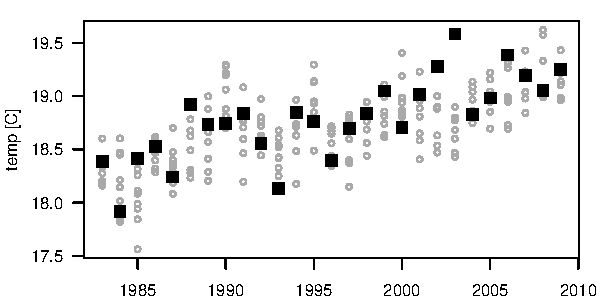
\includegraphics{fig-gfs-plot}
%
\end{center}
\caption{Seasonal European temperature forecasts by NCEP CFSv2, initialised in May, verified in JJA.}
\label{gfs-plot}
\end{figure}


\section{Ensemble-adjusted verification scores}

\subsection{Representation of ensemble and observation data}

In \pkg{SpecsVerification}, archives of $N$ instances of ensemble forecasts, each with $R$ members, are represented by $N\times R$ matrices.
The data shown in Figure \ref{gfs-plot} is a matrix with dimensions

\begin{Hchunk}
\begin{normalsize}
\begin{Hinput}

\ttfamily\noindent
\hlprompt{{\ }}\hlfunctioncall{dim}\hlkeyword{(}\hlsymbol{ens}\hlkeyword{)}\mbox{}
\normalfont

\end{Hinput}

\begin{Houtput}

\ttfamily\noindent
[1]{\ }27{\ }{\ }8\hspace*{\fill}\hlstd{}\mbox{}
\normalfont

\end{Houtput}

\end{normalsize}
\end{Hchunk}



\subsection{Binary forecasts}

This section outlines the theory behind ensemble-adjusted verification scores, using probabilistic forecasts of binary events for illustration.  

One of the most common verification measures for probabilistic forecasts of binary events is the Brier score \citep{brier1950verification}.
Suppose a probability forecast $p_t \in [0,1]$ is issued at time $t$ for a binary (yes/no) event.
The occurrence or non-occurrence of the event is coded as $y_t=1$ or $y_t=0$, respectively. 
The Brier score is given by the squared difference between forecast and observation:
%
\begin{equation}
s_{B}(p_t, y_t) = (p_t - y_t)^2
\end{equation}
%
The Brier score is negatively oriented - lower scores indicate better forecasts.
The Brier score is a strictly proper verification score, meaning that the expected score obtains its minimum value if and only if the observation $y_t$ is a random draw from $p_t$ \citep{gneiting2007strictly}.


Assume next that instead of predicting the probability $p_t$, we make a prediction based on an ensemble forecast of size $R$, whose members were sampled identically and independently with probability $p_t$.
That is, each of the $R$ ensemble members is an independent Bernoulli trial with success probability $p_t$.
An unbiased estimator of the success probability $p_t$ is given by the fraction $i_t/R$, where $i_t$ is the number of successes, i.e. the number of ensemble members that predict the event $y_t=1$.
The Brier score of the estimated probability is equal to
%
\begin{equation}
s_{B}\left(\frac{i_t}{R}, y_t\right) = \left(\frac{i_t}{R} - y_t\right)^2
\label{eq:unfair-brier}
\end{equation}
%
Taking expectation over the random variable $i_t \sim Binomial(p_t, R)$, it is shown that \citep{ferro2008effect}
%
\begin{equation}
E\left[s_{B}\left(\frac{i_t}{R}, y_t\right)\right] = s_{B}(p_t, y_t) +\frac{p_t(1-p_t)}{R}
\label{eq:expec-brier}
\end{equation}
%
That is, even though the fraction $i_t/R$ is an unbiased estimator of the event probability $p_t$, the Brier score of $i_t/R$ is not an unbiased estimator of the Brier score of $p_t$.
The bias, given by the additional positive term on the rhs of Equation~\ref{eq:expec-brier}, depends on the ensemble size and vanishes for $R\rightarrow\infty$.
The bias can be interpreted as a finite-ensemble penalty: If two ensembles sample their members from the same probability $p_t$, the one with the larger ensemble size obtains the lower (i.e. better) Brier score on average.
This is reasonable since more ensemble members allow for more robust estimation of the ``true'' probability $p_t$.
But in the analysis of ensemble hindcasts it is sometimes desirable to correct the finite-ensemble bias.
For example, if the hindcast ensemble has $R$ members, and future operational forecasts will be made with $R^* > R$ ensemble members, the score calculated for the $R$-member hindcast ensemble will be a too pessimistic estimate of the score of the $R^*$-member forecast ensemble.


The ensemble-adjusted Brier score, given by \citep{ferro2008effect}
%
\begin{equation}
s_{B}^*(i_t, R, R^*, y_t) = \left(\frac{i_t}{R} - y_t\right)^2 - \frac{i_t(R-i_t)}{R(R-1)}\left(\frac{1}{R} - \frac{1}{R^*}\right)
\label{eq:ens-brier}
\end{equation}
%
allows to correct the finite-ensemble bias.
The ensemble-adjusted Brier score is is in expectation equal to the Brier score that would be achieved by an ensemble with $R^*$ members sampled from the same probability $p_t$, i.e., 
%
\begin{equation}
E\left[s_{B}^*(i_t, R, R^*, y_t)\right] = (p_t - y_t)^2 + \frac{p_t(1-p_t)}{R^*}.
\end{equation}
%
Note that, trivially, $s_{B}^*(i_t, R, R, y_t) = s_{B}(i_t/R, y_t)$.
Note further that setting $R^*=\infty$ yields the fair Brier score \citep{ferro2013fair} which estimates the score of the underlying probability $p_t$.
The ensemble-adjusted Brier score can be used to compare ensemble forecasting systems with different numbers of members.
It further allows for the extrapolation of the average score of an ensemble forecast system to larger ensemble sizes.


The \pkg{SpecsVerification} function \code{EnsBrier} calculates the ensemble-adjusted Brier scores of a collection of $N$ ensemble forecasts and their corresponding binary observations. 
The argument \code{R.new} allows for estimation of the score of an arbitrary ensemble size, including \code{R.new=Inf}.


We transform the continuous ensemble data into binary by addressing the question "Will this year's summer be warmer than last year's"?

\begin{Hchunk}
\begin{normalsize}
\begin{Hinput}

\ttfamily\noindent
\hlprompt{{\ }}\hlfunctioncall{rbind}\hlkeyword{(}\hspace*{\fill}\\
\hlstd{}\hlprompt{{\ }}{\ }{\ }\hlargument{unadjusted}{\ }\hlargument{=}{\ }\hlfunctioncall{mean}\hlkeyword{(}\hlfunctioncall{EnsBrier}\hlkeyword{(}\hlsymbol{ens.bin}\hlkeyword{,}{\ }\hlsymbol{obs.bin}\hlkeyword{,}{\ }\hlargument{R.new}\hlargument{=}\hlnumber{NA}\hlkeyword{)}\hlkeyword{)}\hlkeyword{,}\hspace*{\fill}\\
\hlstd{}\hlprompt{{\ }}{\ }{\ }\hlargument{fair}{\ }{\ }{\ }{\ }{\ }{\ }{\ }\hlargument{=}{\ }\hlfunctioncall{mean}\hlkeyword{(}\hlfunctioncall{EnsBrier}\hlkeyword{(}\hlsymbol{ens.bin}\hlkeyword{,}{\ }\hlsymbol{obs.bin}\hlkeyword{,}{\ }\hlargument{R.new}\hlargument{=}\hlnumber{Inf}\hlkeyword{)}\hlkeyword{)}\hspace*{\fill}\\
\hlstd{}\hlprompt{{\ }}\hlkeyword{)}\mbox{}
\normalfont

\end{Hinput}

\begin{Houtput}

\ttfamily\noindent
{\ }{\ }{\ }{\ }{\ }{\ }{\ }{\ }{\ }{\ }{\ }{\ }{\ }[,1]\hspace*{\fill}\\
\hlstd{}unadjusted{\ }0.1753\hspace*{\fill}\\
\hlstd{}fair{\ }{\ }{\ }{\ }{\ }{\ }{\ }0.1534\hspace*{\fill}\hlstd{}\mbox{}
\normalfont

\end{Houtput}

\end{normalsize}
\end{Hchunk}




\subsection{Categorical forecasts}


Assume the ensemble forecasting system produces an ensemble of categorical rather than binary forecasts.
That is, each ensemble members and the verifying observation falls into one of $K$ classes.
Two types of categorical forecasts can be distinguished: Disjoint categories and nested categories.

Assume the observation assumes on of $K$ possible values, or classes, and a probabilistic forecast $\mathbf{p}_t = (p_{t,1}, \cdots, p_{t,K})$, is issued.
The verifying observation is vector-valued $\mathbf{y}_t$, where the $k$-th element of $\mathbf{y}_t$ is $y_{t,k}=1$ if the $k$-th class is observed, and $y_{t,k}=0$ otherwise.
The quadratic score for such a probability forecast is given by
%
\begin{equation}
s_{Q}(\mathbf{p}_t, \mathbf{y}_t) = \sum_{k=1}^K \left(p_{t,k} - y_{t,k}\right)^2
\end{equation}
%
The quadratic score is simply the sum of Brier scores for the individual categories.
Or stated differently, the Brier score is one-half the quadratic score of a 2-class categorical forecast.

Now assume an $R$-member categorical ensemble forecast $\mathbf{i}_t$ is issued at time $t$, indicating that $i_{t,k}$ out of $R$ ensemble members have predicted the $k$-th category, for $k=1,\cdots,K$.
Using results obtained for the ensemble-adjusted Brier score, the ensemble-adjusted quadratic score is seen to be
%
\begin{equation}
s_{Q}^*(\mathbf{i}_t, R, R^*, \mathbf{y}_t) = \sum_{k=1}^K \left\{ \left(\frac{i_{t,k}}{R} - y_{t,k}\right)^2 - \left(\frac{1}{R} - \frac{1}{R^*}\right) \frac{i_{t,k}(R-i_{t,k})}{R(R-1)}\right\}
\end{equation}
%
The ensemble adjusted quadratic score is implemented as the function \code{EnsQs} in \pkg{SpecsVerification}.


The quadratic score is insensitive to relabelling the $K$ categories.
Sometimes this is undesired in categorical forecasting problems. 
The forecast categories might have a natural ordering, such as low/medium/high intensity of precipitation.
In that case, an order-sensitive score might be desired that penalises forecasts that assign most probability to the ``high'' category more than it penalises forecasts that assign most probability to the ``medium'' category, if the low category verifies. 
A lot of probability in the ``medium'' category can be considered closer to the observation than a lot of probability in the ``high'' category, such that the former forecast can be considered ``better''.
An order-sensitive score is also desired if the forecast categories are nested within one another, e.g., for precipitation amounts categorised into <1mm/<5mm/<20mm/<$\infty$.
In that case, a high probability assigned to the <5mm category should receive less penalty than a high probability assigned to the <20mm category, if the actual amount is <1mm.


The ranked probability score (RPS) is an order-sensitive quadratic score for categorical probability forecasts.
The forecast vector $\mathbf{i}_t$ is transformed to the $K$-element cumulated forecast vector $\mathbf{j}_t$, with $k$-th element equal to $j_{t,k} = \sum_{l=1}^k i_{t,l}$.
Likewise, the cumulated observation vector $\mathbf{z}_t$ has its $k$-th element equal to $z_{t,k} = \sum_{l=1}^k y_{t,l}$.
The RPS is the quadratic score achieved by the cumulative forecast $\mathbf{j}_t$ for the cumulative observation $\mathbf{z}_t$.
Accumulating the elements of $\mathbf{i}_t$ and $\mathbf{y}_t$ nests the $K$ forecast categories within each other. 
The forecast is transformed from ``$i_{t,k}$ out of $R$ ensemble members predict category $k$'' to the forecast ``$j_{t,k}$ out of $R$ ensemble members forecast category $k$ \emph{or less}''.
The nesting of forecast categories ensures order-sensitivity of the score.
Using results from the previous section, we get the ensemble-adjusted RPS
%
\begin{equation}
s_{R}^*(\mathbf{i}_t, R, R^*, \mathbf{y}_t) = \sum_{k=1}^K \left\{ \left(\frac{j_{t,k}}{R} - z_{t,k}\right)^2 - \left(\frac{1}{R} - \frac{1}{R^*}\right) \frac{j_{t,k}(R-j_{t,k})}{R(R-1)}\right\}
\end{equation}
%
The ensemble adjusted RPS is implemented as the function \code{EnsRps} in \pkg{SpecsVerification}.



We transform the continuous ensemble forecasts into categorical forecasts by addressing the question "Will this year's summer temperature be similar to last year's temperature (within a 0.5K range), colder, or warmer?"

\begin{Hchunk}
\begin{normalsize}
\begin{Hinput}

\ttfamily\noindent
\hlprompt{{\ }}\hlfunctioncall{cbind}\hlkeyword{(}\hspace*{\fill}\\
\hlstd{}\hlprompt{{\ }}\hlargument{qs}{\ }\hlargument{=}{\ }\hlfunctioncall{c}\hlkeyword{(}\hspace*{\fill}\\
\hlstd{}\hlprompt{{\ }}{\ }{\ }\hlargument{unadjusted}{\ }\hlargument{=}{\ }\hlfunctioncall{mean}\hlkeyword{(}\hlfunctioncall{EnsQs}\hlkeyword{(}\hlsymbol{ens.cat}\hlkeyword{,}{\ }\hlsymbol{obs.cat}\hlkeyword{,}{\ }\hlargument{R.new}\hlargument{=}\hlnumber{NA}\hlkeyword{)}\hlkeyword{)}\hlkeyword{,}\hspace*{\fill}\\
\hlstd{}\hlprompt{{\ }}{\ }{\ }\hlargument{fair}{\ }{\ }{\ }{\ }{\ }{\ }{\ }\hlargument{=}{\ }\hlfunctioncall{mean}\hlkeyword{(}\hlfunctioncall{EnsQs}\hlkeyword{(}\hlsymbol{ens.cat}\hlkeyword{,}{\ }\hlsymbol{obs.cat}\hlkeyword{,}{\ }\hlargument{R.new}\hlargument{=}\hlnumber{Inf}\hlkeyword{)}\hlkeyword{)}\hspace*{\fill}\\
\hlstd{}\hlprompt{{\ }}\hlkeyword{)}\hlkeyword{,}\hspace*{\fill}\\
\hlstd{}\hlprompt{{\ }}\hlargument{rps}{\ }\hlargument{=}{\ }\hlfunctioncall{c}\hlkeyword{(}\hspace*{\fill}\\
\hlstd{}\hlprompt{{\ }}{\ }{\ }\hlargument{unadjusted}{\ }\hlargument{=}{\ }\hlfunctioncall{mean}\hlkeyword{(}\hlfunctioncall{EnsRps}\hlkeyword{(}\hlsymbol{ens.cat}\hlkeyword{,}{\ }\hlsymbol{obs.cat}\hlkeyword{,}{\ }\hlargument{R.new}\hlargument{=}\hlnumber{NA}\hlkeyword{)}\hlkeyword{)}\hlkeyword{,}\hspace*{\fill}\\
\hlstd{}\hlprompt{{\ }}{\ }{\ }\hlargument{fair}{\ }{\ }{\ }{\ }{\ }{\ }{\ }\hlargument{=}{\ }\hlfunctioncall{mean}\hlkeyword{(}\hlfunctioncall{EnsRps}\hlkeyword{(}\hlsymbol{ens.cat}\hlkeyword{,}{\ }\hlsymbol{obs.cat}\hlkeyword{,}{\ }\hlargument{R.new}\hlargument{=}\hlnumber{Inf}\hlkeyword{)}\hlkeyword{)}\hspace*{\fill}\\
\hlstd{}\hlprompt{{\ }}\hlkeyword{)}\hlkeyword{)}\mbox{}
\normalfont

\end{Hinput}

\begin{Houtput}

\ttfamily\noindent
{\ }{\ }{\ }{\ }{\ }{\ }{\ }{\ }{\ }{\ }{\ }{\ }{\ }{\ }{\ }qs{\ }{\ }{\ }{\ }rps\hspace*{\fill}\\
\hlstd{}unadjusted{\ }0.6389{\ }0.3843\hspace*{\fill}\\
\hlstd{}fair{\ }{\ }{\ }{\ }{\ }{\ }{\ }0.5873{\ }0.3752\hspace*{\fill}\hlstd{}\mbox{}
\normalfont

\end{Houtput}

\end{normalsize}
\end{Hchunk}





\subsection{Continuous forecasts}


If the forecast target is a continuous variable, such as temperature or pressure, the continuous ranked probability score \citep{matheson1976scoring} can be used for forecast verification.
If the forecast for the continuous target $y_t$ is given as a cumulative distribution function $F_t(x)$, the CRPS is given by 
%
\begin{equation}
s_{C}(F_t, y_t) = \int_{-\infty}^\infty dz\ \left[F_t(z) - H(z-y_t)\right]^2
\end{equation}
%
where $H(x)$ is the Heaviside step-function, satisfying $H(x)=1$ for all $x\ge 0$ and $H(x)=0$ otherwise.
Suppose an ensemble forecast $x_t$ with $R$ real-valued members $x_t = \{x_{t,1}, x_{t,2} \dots, x_{t,R}\}$ is issued for the real-valued verifying observation $y_t$.
The ensemble can be transformed into a cdf by taking the empirical distribution function given by 
%
\begin{equation}
\hat{F}_t(z) = \frac{1}{R} \sum_{r=1}^{R} H(z - x_{t,r}).
\end{equation}
%
Using properties of the Heaviside function, it is straightforward to show that the CRPS of the empirical distribution $\hat{F}$ is given by
%
\begin{equation}
s_{C}(\hat{F}_t, y_t) = \frac{1}{R}|x_{t,r}-y_t| - \frac{1}{2R^2} \sum_{r=1}^R \sum_{r'=1}^R |x_{t,r}-x_{t,r'}|.
\end{equation}
%
\citet{fricker2013three} show that the CRPS is sensitive with respect to the ensemble size, and propose the ensemble-adjusted CRPS
%
\begin{equation}
s_{C}^*(x_t, R, R^*, y_t) = \frac{1}{R}\sum_{r=1}^R |x_{t,r} - y_t| - \frac{1}{2R(R-1)}\left(1-\frac{1}{R^*}\right) \sum_{r=1}^R\sum_{r'=1}^R |x_{t,r}-x_{t,r'}|.
\end{equation}
%
The ensemble-adjusted CRPS is, in expectation, equal to the CRPS that the empirical distribution function calculated from an ensemble of size $R^*$ would achieve.
This includes the case $R^*=\infty$, for which the fair CRPS is obtained.
The ensemble-adjusted CRPS is implemented in the \pkg{SpecsVerification} function \code{EnsCrps}.

\begin{Hchunk}
\begin{normalsize}
\begin{Hinput}

\ttfamily\noindent
\hlprompt{{\ }}\hlfunctioncall{rbind}\hlkeyword{(}\hspace*{\fill}\\
\hlstd{}\hlprompt{{\ }}{\ }{\ }\hlargument{unadjusted}{\ }\hlargument{=}{\ }\hlfunctioncall{mean}\hlkeyword{(}\hlfunctioncall{EnsCrps}\hlkeyword{(}\hlsymbol{ens}\hlkeyword{,}{\ }\hlsymbol{obs}\hlkeyword{,}{\ }\hlargument{R.new}\hlargument{=}\hlnumber{NA}\hlkeyword{)}\hlkeyword{)}\hlkeyword{,}\hspace*{\fill}\\
\hlstd{}\hlprompt{{\ }}{\ }{\ }\hlargument{fair}{\ }{\ }{\ }{\ }{\ }{\ }{\ }\hlargument{=}{\ }\hlfunctioncall{mean}\hlkeyword{(}\hlfunctioncall{EnsCrps}\hlkeyword{(}\hlsymbol{ens}\hlkeyword{,}{\ }\hlsymbol{obs}\hlkeyword{,}{\ }\hlargument{R.new}\hlargument{=}\hlnumber{Inf}\hlkeyword{)}\hlkeyword{)}\hspace*{\fill}\\
\hlstd{}\hlprompt{{\ }}\hlkeyword{)}\mbox{}
\normalfont

\end{Hinput}

\begin{Houtput}

\ttfamily\noindent
{\ }{\ }{\ }{\ }{\ }{\ }{\ }{\ }{\ }{\ }{\ }{\ }[,1]\hspace*{\fill}\\
\hlstd{}unadjusted{\ }0.165\hspace*{\fill}\\
\hlstd{}fair{\ }{\ }{\ }{\ }{\ }{\ }{\ }0.150\hspace*{\fill}\hlstd{}\mbox{}
\normalfont

\end{Houtput}

\end{normalsize}
\end{Hchunk}



The ensemble adjusted Ignorance score has recently been proposed \citep{siegert2015ignorance}.





\section{Comparative verification and uncertainty quantification}


\subsection{Reference forecast}

The value of a verification score by itself is meaningless.
In order to evaluate the skill of a forecast, its verification score has to be compared to the score achieved by a reference forecast.
For example, if the skill of a state-of-the-art high resolution climate model is evaluated, it is reasonable to compare its verification score to the score achieved by an older climate model, possibly with lower resolution and less physical detail.

In the absence of a dynamical climate model to which the score can be compared, simple statistical benchmark predictions can be used.
A popular simple reference forecast is the climatological forecast, which is only based on the known record of observations, without reference to any numerical forecast model.
\pkg{SpecsVerification} includes the function \code{ClimEns} which transforms a vector of observations into a matrix of climatological ensemble forecasts, including the possibility to leave out the $t$-th observation in the $t$-th climatological ensemble:

\begin{Hchunk}
\begin{normalsize}
\begin{Hinput}

\ttfamily\noindent
\hlprompt{{\ }}\hlsymbol{ens.ref}{\ }{\ }{\ }{\ }{\ }\hlassignement{\usebox{\hlnormalsizeboxlessthan}-}{\ }\hlfunctioncall{ClimEns}\hlkeyword{(}\hlsymbol{obs}\hlkeyword{,}{\ }{\ }{\ }{\ }{\ }\hlargument{leave.one.out}\hlargument{=}\hlnumber{TRUE}\hlkeyword{)}\mbox{}
\normalfont

\end{Hinput}


\begin{Hinput}

\ttfamily\noindent
\hlprompt{{\ }}\hlsymbol{ens.cat.ref}{\ }\hlassignement{\usebox{\hlnormalsizeboxlessthan}-}{\ }\hlfunctioncall{ClimEns}\hlkeyword{(}\hlsymbol{obs.cat}\hlkeyword{,}{\ }\hlargument{leave.one.out}\hlargument{=}\hlnumber{TRUE}\hlkeyword{)}\mbox{}
\normalfont

\end{Hinput}


\begin{Hinput}

\ttfamily\noindent
\hlprompt{{\ }}\hlsymbol{ens.bin.ref}{\ }\hlassignement{\usebox{\hlnormalsizeboxlessthan}-}{\ }\hlfunctioncall{ClimEns}\hlkeyword{(}\hlsymbol{obs.bin}\hlkeyword{,}{\ }\hlargument{leave.one.out}\hlargument{=}\hlnumber{TRUE}\hlkeyword{)}\mbox{}
\normalfont

\end{Hinput}


\end{normalsize}
\end{Hchunk}


The new data set of climatological ensembles can be used as a reference ensemble to which the numerical forecast ensemble can be compared.
We recommend also considering statistical reference forecasts such as a linear trend or an auto-regressive model, which might be more suitable than the climatological forecast.



\subsection{Mean scores and mean score differences}

Suppose we have calculated two time series $\{s_{1,1}, s_{1,2}, \dots, s_{1,N}\}$ and $\{s_{2,1}, s_{2,2}, \dots, s_{2,N}\}$ of verification scores for two competing forecast systems for the same observation.
\citet{diebold1995comparing} suggest to test the null-hypothesis of equal forecast accuracy using the time series $d_1, \dots, d_N$ of loss differentials $d_t = s_{1,t} - s_{2,t}$. 
Under the assumption of temporal independence of $d_t$, and zero mean of the loss-differential, the test statistic 
%
\begin{equation}
T = \bar{d}\sqrt{\frac{N}{var(d_t)}}
\end{equation}
%
is asymptotically Normally distributed with mean zero and variance one.
This test is implemented in \pkg{SpecsVerification} in the function \code{ScoreDiff}.
The function includes the option to account for autocorrelation of the loss-differential by specifying an effective sample size \code{N.eff}.

\begin{Hchunk}
\begin{normalsize}
\begin{Hinput}

\ttfamily\noindent
\hlprompt{{\ }}\hlfunctioncall{rbind}\hlkeyword{(}\hspace*{\fill}\\
\hlstd{}\hlprompt{{\ }}{\ }{\ }\hlargument{brier}{\ }\hlargument{=}{\ }\hlfunctioncall{ScoreDiff}\hlkeyword{(}\hlfunctioncall{EnsBrier}\hlkeyword{(}\hlsymbol{ens.bin}\hlkeyword{,}{\ }\hlsymbol{obs.bin}\hlkeyword{)}\hlkeyword{,}\hspace*{\fill}\\
\hlstd{}\hlprompt{{\ }}{\ }{\ }{\ }{\ }{\ }{\ }{\ }{\ }{\ }{\ }{\ }{\ }{\ }{\ }{\ }{\ }{\ }{\ }{\ }{\ }\hlfunctioncall{EnsBrier}\hlkeyword{(}\hlsymbol{ens.bin.ref}\hlkeyword{,}{\ }\hlsymbol{obs.bin}\hlkeyword{)}\hlkeyword{)}\hlkeyword{,}\hspace*{\fill}\\
\hlstd{}\hlprompt{{\ }}{\ }{\ }\hlargument{qs}{\ }{\ }{\ }{\ }\hlargument{=}{\ }\hlfunctioncall{ScoreDiff}\hlkeyword{(}\hlfunctioncall{EnsQs}\hlkeyword{(}\hlsymbol{ens.cat}\hlkeyword{,}{\ }\hlsymbol{obs.cat}\hlkeyword{)}\hlkeyword{,}\hspace*{\fill}\\
\hlstd{}\hlprompt{{\ }}{\ }{\ }{\ }{\ }{\ }{\ }{\ }{\ }{\ }{\ }{\ }{\ }{\ }{\ }{\ }{\ }{\ }{\ }{\ }{\ }\hlfunctioncall{EnsQs}\hlkeyword{(}\hlsymbol{ens.cat.ref}\hlkeyword{,}{\ }\hlsymbol{obs.cat}\hlkeyword{)}\hlkeyword{)}\hlkeyword{,}\hspace*{\fill}\\
\hlstd{}\hlprompt{{\ }}{\ }{\ }\hlargument{rps}{\ }{\ }{\ }\hlargument{=}{\ }\hlfunctioncall{ScoreDiff}\hlkeyword{(}\hlfunctioncall{EnsRps}\hlkeyword{(}\hlsymbol{ens.cat}\hlkeyword{,}{\ }\hlsymbol{obs.cat}\hlkeyword{)}\hlkeyword{,}\hspace*{\fill}\\
\hlstd{}\hlprompt{{\ }}{\ }{\ }{\ }{\ }{\ }{\ }{\ }{\ }{\ }{\ }{\ }{\ }{\ }{\ }{\ }{\ }{\ }{\ }{\ }{\ }\hlfunctioncall{EnsRps}\hlkeyword{(}\hlsymbol{ens.cat.ref}\hlkeyword{,}{\ }\hlsymbol{obs.cat}\hlkeyword{)}\hlkeyword{)}\hlkeyword{,}\hspace*{\fill}\\
\hlstd{}\hlprompt{{\ }}{\ }{\ }\hlargument{crps}{\ }{\ }\hlargument{=}{\ }\hlfunctioncall{ScoreDiff}\hlkeyword{(}\hlfunctioncall{EnsCrps}\hlkeyword{(}\hlsymbol{ens}\hlkeyword{,}{\ }\hlsymbol{obs}\hlkeyword{)}\hlkeyword{,}\hspace*{\fill}\\
\hlstd{}\hlprompt{{\ }}{\ }{\ }{\ }{\ }{\ }{\ }{\ }{\ }{\ }{\ }{\ }{\ }{\ }{\ }{\ }{\ }{\ }{\ }{\ }{\ }\hlfunctioncall{EnsCrps}\hlkeyword{(}\hlsymbol{ens.ref}\hlkeyword{,}{\ }\hlsymbol{obs}\hlkeyword{)}\hlkeyword{)}\hspace*{\fill}\\
\hlstd{}\hlprompt{{\ }}\hlkeyword{)}\mbox{}
\normalfont

\end{Hinput}

\begin{Houtput}

\ttfamily\noindent
{\ }{\ }{\ }{\ }{\ }{\ }score.diff{\ }score.diff.sd{\ }p.value{\ }{\ }{\ }{\ }{\ }{\ }ci.L{\ }{\ }{\ }ci.U\hspace*{\fill}\\
\hlstd{}brier{\ }{\ }{\ }{\ }0.08501{\ }{\ }{\ }{\ }{\ }{\ }{\ }0.05950{\ }0.07656{\ }-0.031619{\ }0.2016\hspace*{\fill}\\
\hlstd{}qs{\ }{\ }{\ }{\ }{\ }{\ }{\ }0.05934{\ }{\ }{\ }{\ }{\ }{\ }{\ }0.09683{\ }0.27000{\ }-0.130438{\ }0.2491\hspace*{\fill}\\
\hlstd{}rps{\ }{\ }{\ }{\ }{\ }{\ }0.04769{\ }{\ }{\ }{\ }{\ }{\ }{\ }0.07477{\ }0.26178{\ }-0.098851{\ }0.1942\hspace*{\fill}\\
\hlstd{}crps{\ }{\ }{\ }{\ }{\ }0.06698{\ }{\ }{\ }{\ }{\ }{\ }{\ }0.03126{\ }0.01606{\ }{\ }0.005716{\ }0.1282\hspace*{\fill}\hlstd{}\mbox{}
\normalfont

\end{Houtput}

\end{normalsize}
\end{Hchunk}



How do the score differences change if adjust the ensemble size to infinity?

\begin{Hchunk}
\begin{normalsize}
\begin{Hinput}

\ttfamily\noindent
\hlprompt{{\ }}\hlfunctioncall{rbind}\hlkeyword{(}\hspace*{\fill}\\
\hlstd{}\hlprompt{{\ }}{\ }{\ }\hlargument{brier}{\ }\hlargument{=}{\ }\hlfunctioncall{ScoreDiff}\hlkeyword{(}\hlfunctioncall{EnsBrier}\hlkeyword{(}\hlsymbol{ens.bin}\hlkeyword{,}{\ }{\ }{\ }{\ }{\ }\hlsymbol{obs.bin}\hlkeyword{,}{\ }\hlargument{R.new}\hlargument{=}\hlnumber{Inf}\hlkeyword{)}\hlkeyword{,}\hspace*{\fill}\\
\hlstd{}\hlprompt{{\ }}{\ }{\ }{\ }{\ }{\ }{\ }{\ }{\ }{\ }{\ }{\ }{\ }{\ }{\ }{\ }{\ }{\ }{\ }{\ }{\ }\hlfunctioncall{EnsBrier}\hlkeyword{(}\hlsymbol{ens.bin.ref}\hlkeyword{,}{\ }\hlsymbol{obs.bin}\hlkeyword{,}{\ }\hlargument{R.new}\hlargument{=}\hlnumber{Inf}\hlkeyword{)}\hlkeyword{)}\hlkeyword{,}\hspace*{\fill}\\
\hlstd{}\hlprompt{{\ }}{\ }{\ }\hlargument{qs}{\ }{\ }{\ }{\ }\hlargument{=}{\ }\hlfunctioncall{ScoreDiff}\hlkeyword{(}\hlfunctioncall{EnsQs}\hlkeyword{(}\hlsymbol{ens.cat}\hlkeyword{,}{\ }{\ }{\ }{\ }{\ }\hlsymbol{obs.cat}\hlkeyword{,}{\ }\hlargument{R.new}\hlargument{=}\hlnumber{Inf}\hlkeyword{)}\hlkeyword{,}\hspace*{\fill}\\
\hlstd{}\hlprompt{{\ }}{\ }{\ }{\ }{\ }{\ }{\ }{\ }{\ }{\ }{\ }{\ }{\ }{\ }{\ }{\ }{\ }{\ }{\ }{\ }{\ }\hlfunctioncall{EnsQs}\hlkeyword{(}\hlsymbol{ens.cat.ref}\hlkeyword{,}{\ }\hlsymbol{obs.cat}\hlkeyword{,}{\ }\hlargument{R.new}\hlargument{=}\hlnumber{Inf}\hlkeyword{)}\hlkeyword{)}\hlkeyword{,}\hspace*{\fill}\\
\hlstd{}\hlprompt{{\ }}{\ }{\ }\hlargument{rps}{\ }{\ }{\ }\hlargument{=}{\ }\hlfunctioncall{ScoreDiff}\hlkeyword{(}\hlfunctioncall{EnsRps}\hlkeyword{(}\hlsymbol{ens.cat}\hlkeyword{,}{\ }{\ }{\ }{\ }{\ }\hlsymbol{obs.cat}\hlkeyword{,}{\ }\hlargument{R.new}\hlargument{=}\hlnumber{Inf}\hlkeyword{)}\hlkeyword{,}\hspace*{\fill}\\
\hlstd{}\hlprompt{{\ }}{\ }{\ }{\ }{\ }{\ }{\ }{\ }{\ }{\ }{\ }{\ }{\ }{\ }{\ }{\ }{\ }{\ }{\ }{\ }{\ }\hlfunctioncall{EnsRps}\hlkeyword{(}\hlsymbol{ens.cat.ref}\hlkeyword{,}{\ }\hlsymbol{obs.cat}\hlkeyword{,}{\ }\hlargument{R.new}\hlargument{=}\hlnumber{Inf}\hlkeyword{)}\hlkeyword{)}\hlkeyword{,}\hspace*{\fill}\\
\hlstd{}\hlprompt{{\ }}{\ }{\ }\hlargument{crps}{\ }{\ }\hlargument{=}{\ }\hlfunctioncall{ScoreDiff}\hlkeyword{(}\hlfunctioncall{EnsCrps}\hlkeyword{(}\hlsymbol{ens}\hlkeyword{,}{\ }{\ }{\ }{\ }{\ }\hlsymbol{obs}\hlkeyword{,}{\ }\hlargument{R.new}\hlargument{=}\hlnumber{Inf}\hlkeyword{)}\hlkeyword{,}\hspace*{\fill}\\
\hlstd{}\hlprompt{{\ }}{\ }{\ }{\ }{\ }{\ }{\ }{\ }{\ }{\ }{\ }{\ }{\ }{\ }{\ }{\ }{\ }{\ }{\ }{\ }{\ }\hlfunctioncall{EnsCrps}\hlkeyword{(}\hlsymbol{ens.ref}\hlkeyword{,}{\ }\hlsymbol{obs}\hlkeyword{,}{\ }\hlargument{R.new}\hlargument{=}\hlnumber{Inf}\hlkeyword{)}\hlkeyword{)}\hspace*{\fill}\\
\hlstd{}\hlprompt{{\ }}\hlkeyword{)}\mbox{}
\normalfont

\end{Hinput}

\begin{Houtput}

\ttfamily\noindent
{\ }{\ }{\ }{\ }{\ }{\ }score.diff{\ }score.diff.sd{\ }{\ }p.value{\ }{\ }{\ }{\ }{\ }ci.L{\ }{\ }{\ }ci.U\hspace*{\fill}\\
\hlstd{}brier{\ }{\ }{\ }{\ }0.09727{\ }{\ }{\ }{\ }{\ }{\ }{\ }0.05979{\ }0.051890{\ }-0.01992{\ }0.2145\hspace*{\fill}\\
\hlstd{}qs{\ }{\ }{\ }{\ }{\ }{\ }{\ }0.08506{\ }{\ }{\ }{\ }{\ }{\ }{\ }0.09664{\ }0.189383{\ }-0.10435{\ }0.2745\hspace*{\fill}\\
\hlstd{}rps{\ }{\ }{\ }{\ }{\ }{\ }0.05140{\ }{\ }{\ }{\ }{\ }{\ }{\ }0.07490{\ }0.246276{\ }-0.09540{\ }0.1982\hspace*{\fill}\\
\hlstd{}crps{\ }{\ }{\ }{\ }{\ }0.07344{\ }{\ }{\ }{\ }{\ }{\ }{\ }0.03128{\ }0.009445{\ }{\ }0.01213{\ }0.1347\hspace*{\fill}\hlstd{}\mbox{}
\normalfont

\end{Houtput}

\end{normalsize}
\end{Hchunk}



\subsection{Skill scores}

It is common practice to compare scores of competing forecasts by a so-called skill score, which is a normalised mean score difference \citep{wilks2011statistical}.
Denote by $S$ the mean score of the forecast under evaluation, by $S_{ref}$ the mean score of a reference forecast, and by $S_{perf}$ the mean score that would be achieved by the perfect forecaster.
The skill score is then given by the score difference between the reference forecast and the evaluated forecast, normalised by the difference between the reference forecast and the perfect forecast:
%
\begin{equation}
SS = \frac{S_{ref} - S}{S_{ref} - S_{perf}}
\end{equation}
%
The variance of the skill score can be estimated by error propagation as follows
%
\begin{equation}
var(SS) \approx \frac{1}{(S_{ref} - S_{perf})^2} var(S) + \frac{(S - S_{perf})^2}{(S_{ref}-S_{perf})^2} var(S_{ref}) - 2 \frac{S-S_{perf}}{(S_{ref}-S_{perf})^3} cov(S, S_{ref})
\end{equation}
%
where the variances and covariances of the mean scores are approximated by the variances and covariances of the scores, divided by the sample size.
The skill score is implemented in \pkg{SpecsVerification} in the function \code{SkillScore}, which takes as inputs two vectors of verification scores of the evaluated and the reference forecast, the constant score achieved by a perfect forecaster, as well as a possibly user-defined effective sample size.


\begin{Hchunk}
\begin{normalsize}
\begin{Hinput}

\ttfamily\noindent
\hlprompt{{\ }}\hlfunctioncall{rbind}\hlkeyword{(}\hspace*{\fill}\\
\hlstd{}\hlprompt{{\ }}{\ }{\ }\hlargument{brier}{\ }\hlargument{=}{\ }\hlfunctioncall{SkillScore}\hlkeyword{(}\hlfunctioncall{EnsBrier}\hlkeyword{(}\hlsymbol{ens.bin}\hlkeyword{,}{\ }\hlsymbol{obs.bin}\hlkeyword{)}\hlkeyword{,}\hspace*{\fill}\\
\hlstd{}\hlprompt{{\ }}{\ }{\ }{\ }{\ }{\ }{\ }{\ }{\ }{\ }{\ }{\ }{\ }{\ }{\ }{\ }{\ }{\ }{\ }{\ }{\ }{\ }\hlfunctioncall{EnsBrier}\hlkeyword{(}\hlsymbol{ens.bin.ref}\hlkeyword{,}{\ }\hlsymbol{obs.bin}\hlkeyword{)}\hlkeyword{)}\hlkeyword{,}\hspace*{\fill}\\
\hlstd{}\hlprompt{{\ }}{\ }{\ }\hlargument{qs}{\ }{\ }{\ }{\ }\hlargument{=}{\ }\hlfunctioncall{SkillScore}\hlkeyword{(}\hlfunctioncall{EnsQs}\hlkeyword{(}\hlsymbol{ens.cat}\hlkeyword{,}{\ }\hlsymbol{obs.cat}\hlkeyword{)}\hlkeyword{,}\hspace*{\fill}\\
\hlstd{}\hlprompt{{\ }}{\ }{\ }{\ }{\ }{\ }{\ }{\ }{\ }{\ }{\ }{\ }{\ }{\ }{\ }{\ }{\ }{\ }{\ }{\ }{\ }{\ }\hlfunctioncall{EnsQs}\hlkeyword{(}\hlsymbol{ens.cat.ref}\hlkeyword{,}{\ }\hlsymbol{obs.cat}\hlkeyword{)}\hlkeyword{)}\hlkeyword{,}\hspace*{\fill}\\
\hlstd{}\hlprompt{{\ }}{\ }{\ }\hlargument{rps}{\ }{\ }{\ }\hlargument{=}{\ }\hlfunctioncall{SkillScore}\hlkeyword{(}\hlfunctioncall{EnsRps}\hlkeyword{(}\hlsymbol{ens.cat}\hlkeyword{,}{\ }\hlsymbol{obs.cat}\hlkeyword{)}\hlkeyword{,}\hspace*{\fill}\\
\hlstd{}\hlprompt{{\ }}{\ }{\ }{\ }{\ }{\ }{\ }{\ }{\ }{\ }{\ }{\ }{\ }{\ }{\ }{\ }{\ }{\ }{\ }{\ }{\ }{\ }\hlfunctioncall{EnsRps}\hlkeyword{(}\hlsymbol{ens.cat.ref}\hlkeyword{,}{\ }\hlsymbol{obs.cat}\hlkeyword{)}\hlkeyword{)}\hlkeyword{,}\hspace*{\fill}\\
\hlstd{}\hlprompt{{\ }}{\ }{\ }\hlargument{crps}{\ }{\ }\hlargument{=}{\ }\hlfunctioncall{SkillScore}\hlkeyword{(}\hlfunctioncall{EnsCrps}\hlkeyword{(}\hlsymbol{ens}\hlkeyword{,}{\ }\hlsymbol{obs}\hlkeyword{)}\hlkeyword{,}\hspace*{\fill}\\
\hlstd{}\hlprompt{{\ }}{\ }{\ }{\ }{\ }{\ }{\ }{\ }{\ }{\ }{\ }{\ }{\ }{\ }{\ }{\ }{\ }{\ }{\ }{\ }{\ }{\ }\hlfunctioncall{EnsCrps}\hlkeyword{(}\hlsymbol{ens.ref}\hlkeyword{,}{\ }\hlsymbol{obs}\hlkeyword{)}\hlkeyword{)}\hspace*{\fill}\\
\hlstd{}\hlprompt{{\ }}\hlkeyword{)}\mbox{}
\normalfont

\end{Hinput}

\begin{Houtput}

\ttfamily\noindent
{\ }{\ }{\ }{\ }{\ }{\ }skillscore{\ }skillscore.sd\hspace*{\fill}\\
\hlstd{}brier{\ }{\ }{\ }{\ }0.32651{\ }{\ }{\ }{\ }{\ }{\ }{\ }{\ }0.2152\hspace*{\fill}\\
\hlstd{}qs{\ }{\ }{\ }{\ }{\ }{\ }{\ }0.08498{\ }{\ }{\ }{\ }{\ }{\ }{\ }{\ }0.1400\hspace*{\fill}\\
\hlstd{}rps{\ }{\ }{\ }{\ }{\ }{\ }0.11041{\ }{\ }{\ }{\ }{\ }{\ }{\ }{\ }0.1729\hspace*{\fill}\\
\hlstd{}crps{\ }{\ }{\ }{\ }{\ }0.28872{\ }{\ }{\ }{\ }{\ }{\ }{\ }{\ }0.1183\hspace*{\fill}\hlstd{}\mbox{}
\normalfont

\end{Houtput}

\end{normalsize}
\end{Hchunk}


The skill scores increase slightly if we adjust the ensemble size to $R^* \to \infty$ for the ensemble forecasts and the climatological reference forecast:

\begin{Hchunk}
\begin{normalsize}
\begin{Hinput}

\ttfamily\noindent
\hlprompt{{\ }}\hlfunctioncall{rbind}\hlkeyword{(}\hspace*{\fill}\\
\hlstd{}\hlprompt{{\ }}{\ }{\ }\hlargument{brier}{\ }\hlargument{=}{\ }\hlfunctioncall{SkillScore}\hlkeyword{(}\hlfunctioncall{EnsBrier}\hlkeyword{(}\hlsymbol{ens.bin}\hlkeyword{,}{\ }\hlsymbol{obs.bin}\hlkeyword{,}{\ }\hlargument{R.new}\hlargument{=}\hlnumber{Inf}\hlkeyword{)}\hlkeyword{,}\hspace*{\fill}\\
\hlstd{}\hlprompt{{\ }}{\ }{\ }{\ }{\ }{\ }{\ }{\ }{\ }{\ }{\ }{\ }{\ }{\ }{\ }{\ }{\ }{\ }{\ }{\ }{\ }{\ }\hlfunctioncall{EnsBrier}\hlkeyword{(}\hlsymbol{ens.bin.ref}\hlkeyword{,}{\ }\hlsymbol{obs.bin}\hlkeyword{,}{\ }\hlargument{R.new}\hlargument{=}\hlnumber{Inf}\hlkeyword{)}\hlkeyword{)}\hlkeyword{,}\hspace*{\fill}\\
\hlstd{}\hlprompt{{\ }}{\ }{\ }\hlargument{qs}{\ }{\ }{\ }{\ }\hlargument{=}{\ }\hlfunctioncall{SkillScore}\hlkeyword{(}\hlfunctioncall{EnsQs}\hlkeyword{(}\hlsymbol{ens.cat}\hlkeyword{,}{\ }\hlsymbol{obs.cat}\hlkeyword{,}{\ }\hlargument{R.new}\hlargument{=}\hlnumber{Inf}\hlkeyword{)}\hlkeyword{,}\hspace*{\fill}\\
\hlstd{}\hlprompt{{\ }}{\ }{\ }{\ }{\ }{\ }{\ }{\ }{\ }{\ }{\ }{\ }{\ }{\ }{\ }{\ }{\ }{\ }{\ }{\ }{\ }{\ }\hlfunctioncall{EnsQs}\hlkeyword{(}\hlsymbol{ens.cat.ref}\hlkeyword{,}{\ }\hlsymbol{obs.cat}\hlkeyword{,}{\ }\hlargument{R.new}\hlargument{=}\hlnumber{Inf}\hlkeyword{)}\hlkeyword{)}\hlkeyword{,}\hspace*{\fill}\\
\hlstd{}\hlprompt{{\ }}{\ }{\ }\hlargument{rps}{\ }{\ }{\ }\hlargument{=}{\ }\hlfunctioncall{SkillScore}\hlkeyword{(}\hlfunctioncall{EnsRps}\hlkeyword{(}\hlsymbol{ens.cat}\hlkeyword{,}{\ }\hlsymbol{obs.cat}\hlkeyword{,}{\ }\hlargument{R.new}\hlargument{=}\hlnumber{Inf}\hlkeyword{)}\hlkeyword{,}\hspace*{\fill}\\
\hlstd{}\hlprompt{{\ }}{\ }{\ }{\ }{\ }{\ }{\ }{\ }{\ }{\ }{\ }{\ }{\ }{\ }{\ }{\ }{\ }{\ }{\ }{\ }{\ }{\ }\hlfunctioncall{EnsRps}\hlkeyword{(}\hlsymbol{ens.cat.ref}\hlkeyword{,}{\ }\hlsymbol{obs.cat}\hlkeyword{,}{\ }\hlargument{R.new}\hlargument{=}\hlnumber{Inf}\hlkeyword{)}\hlkeyword{)}\hlkeyword{,}\hspace*{\fill}\\
\hlstd{}\hlprompt{{\ }}{\ }{\ }\hlargument{crps}{\ }{\ }\hlargument{=}{\ }\hlfunctioncall{SkillScore}\hlkeyword{(}\hlfunctioncall{EnsCrps}\hlkeyword{(}\hlsymbol{ens}\hlkeyword{,}{\ }\hlsymbol{obs}\hlkeyword{,}{\ }\hlargument{R.new}\hlargument{=}\hlnumber{Inf}\hlkeyword{)}\hlkeyword{,}\hspace*{\fill}\\
\hlstd{}\hlprompt{{\ }}{\ }{\ }{\ }{\ }{\ }{\ }{\ }{\ }{\ }{\ }{\ }{\ }{\ }{\ }{\ }{\ }{\ }{\ }{\ }{\ }{\ }\hlfunctioncall{EnsCrps}\hlkeyword{(}\hlsymbol{ens.ref}\hlkeyword{,}{\ }\hlsymbol{obs}\hlkeyword{,}{\ }\hlargument{R.new}\hlargument{=}\hlnumber{Inf}\hlkeyword{)}\hlkeyword{)}\hspace*{\fill}\\
\hlstd{}\hlprompt{{\ }}\hlkeyword{)}\mbox{}
\normalfont

\end{Hinput}

\begin{Houtput}

\ttfamily\noindent
{\ }{\ }{\ }{\ }{\ }{\ }skillscore{\ }skillscore.sd\hspace*{\fill}\\
\hlstd{}brier{\ }{\ }{\ }{\ }{\ }0.3880{\ }{\ }{\ }{\ }{\ }{\ }{\ }{\ }0.2225\hspace*{\fill}\\
\hlstd{}qs{\ }{\ }{\ }{\ }{\ }{\ }{\ }{\ }0.1265{\ }{\ }{\ }{\ }{\ }{\ }{\ }{\ }0.1459\hspace*{\fill}\\
\hlstd{}rps{\ }{\ }{\ }{\ }{\ }{\ }{\ }0.1205{\ }{\ }{\ }{\ }{\ }{\ }{\ }{\ }0.1753\hspace*{\fill}\\
\hlstd{}crps{\ }{\ }{\ }{\ }{\ }{\ }0.3287{\ }{\ }{\ }{\ }{\ }{\ }{\ }{\ }0.1215\hspace*{\fill}\hlstd{}\mbox{}
\normalfont

\end{Houtput}

\end{normalsize}
\end{Hchunk}



\subsection{Correlation and correlation difference}

The Pearson correlation coefficient is one of the most popular verification criteria, and can be calculated with the built-in \proglang{R} function \code{cor}.
Since uncertainty quantification is often of interest, \pkg{SpecsVerification} provides the function \code{Corr}, which returns a correlation coefficient, a p-value and a confidence interval.
The user can provide the confidence level for the confidence interval, an effective sample size to account for possible auto-correlation in the data:

\begin{Hchunk}
\begin{normalsize}
\begin{Hinput}

\ttfamily\noindent
\hlprompt{{\ }}\hlsymbol{ens.mean}{\ }\hlassignement{\usebox{\hlnormalsizeboxlessthan}-}{\ }\hlfunctioncall{rowMeans}\hlkeyword{(}\hlsymbol{ens}\hlkeyword{)}\mbox{}
\normalfont

\end{Hinput}


\begin{Hinput}

\ttfamily\noindent
\hlprompt{{\ }}\hlfunctioncall{Corr}\hlkeyword{(}\hlsymbol{ens.mean}\hlkeyword{,}{\ }\hlsymbol{obs}\hlkeyword{)}\mbox{}
\normalfont

\end{Hinput}

\begin{Houtput}

\ttfamily\noindent
{\ }{\ }{\ }{\ }{\ }{\ }corr{\ }{\ }{\ }{\ }p.value{\ }{\ }{\ }{\ }{\ }{\ }{\ }{\ }{\ }{\ }L{\ }{\ }{\ }{\ }{\ }{\ }{\ }{\ }{\ }{\ }U{\ }\hspace*{\fill}\\
\hlstd{}0.67918877{\ }0.00004901{\ }0.40325555{\ }0.84190582{\ }\hspace*{\fill}\hlstd{}\mbox{}
\normalfont

\end{Houtput}

\end{normalsize}
\end{Hchunk}



It is often of interest to compare the correlation coefficients between two forecasts that were issued for the same observation.
The actual difference in correlation is of interest, as well as an estimation of the statistical significance of the correlation difference.
\pkg{SpecsVerification} implements the function \code{CorrDiff} that returns the difference between the correlation of the forecast ensemble \code{ens} and the correlation of a reference forecast ensemble \code{ens.ref}, both of which were issued for the same observation \code{obs}.
The function calculates a p-value using the test by \citet{steiger1980tests} and a confidence interval based on \citet{zou2007toward} are calculated.
Both methods take into account correlation between the two competing forecasts.
For illustration, we evaluate the difference in correlation between the ensemble mean forecast and the persistence forecast:


\begin{Hchunk}
\begin{normalsize}
\begin{Hinput}

\ttfamily\noindent
\hlprompt{{\ }}\hlfunctioncall{CorrDiff}\hlkeyword{(}\hlsymbol{ens.mean}\hlkeyword{,}{\ }\hlsymbol{obs.lag}\hlkeyword{,}{\ }\hlsymbol{obs}\hlkeyword{)}\mbox{}
\normalfont

\end{Hinput}

\begin{Houtput}

\ttfamily\noindent
corr.diff{\ }{\ }{\ }p.value{\ }{\ }{\ }{\ }{\ }{\ }{\ }{\ }{\ }L{\ }{\ }{\ }{\ }{\ }{\ }{\ }{\ }{\ }U{\ }\hspace*{\fill}\\
\hlstd{}{\ }{\ }{\ }0.1011{\ }{\ }{\ }{\ }0.1667{\ }{\ }{\ }-0.1118{\ }{\ }{\ }{\ }0.3532{\ }\hspace*{\fill}\hlstd{}\mbox{}
\normalfont

\end{Houtput}

\end{normalsize}
\end{Hchunk}





\section{Rank histogram analysis for ensemble forecasts}

The verification rank histogram \citep{hamill2001interpretation} is a non-parametric graphical tool to assess the reliability of an ensemble forecasting system.
For each pair of ensemble forecast and verifying observation, the rank of the observation among the ordered ensemble members is calculated.
In a $R$-member ensemble, the rank is between $1$ and $R+1$.
If the ensemble is a reliable representation of the uncertainty in the observation, the observation should statistically behave like ``just another ensemble member''. 
Each verification rank should therefore be equally likely on average, and the histogram over verification ranks should be flat. 
\pkg{SpecsVerification} contains the function \code{Rankhist} to calculate the verification rank counts for an archive of ensembles and observations.

\begin{Hchunk}
\begin{normalsize}
\begin{Hinput}

\ttfamily\noindent
\hlprompt{{\ }}\hlsymbol{rh}{\ }\hlassignement{\usebox{\hlnormalsizeboxlessthan}-}{\ }\hlfunctioncall{Rankhist}\hlkeyword{(}\hlsymbol{ens}\hlkeyword{,}{\ }\hlsymbol{obs}\hlkeyword{)}\mbox{}
\normalfont

\end{Hinput}


\begin{Hinput}

\ttfamily\noindent
\hlprompt{{\ }}\hlsymbol{rh}\mbox{}
\normalfont

\end{Hinput}

\begin{Houtput}

\ttfamily\noindent
[1]{\ }2{\ }3{\ }4{\ }1{\ }2{\ }2{\ }3{\ }5{\ }5\hspace*{\fill}\hlstd{}\mbox{}
\normalfont

\end{Houtput}

\end{normalsize}
\end{Hchunk}




The function \code{PlotRankhist} plots the rank histogram.
Two plotting modes are available:
\code{mode="raw"} simply plots the rank counts as a bar plot histogram.
\code{mode="prob.paper"} plots the rank counts on probability paper following \citet{broecker2008reliability}. 
Assuming that each rank count has a binomial distribution with success probability $1/(R+1)$ and sample size $N$.
The observed rank count $c_i$ is transformed to the cumulative probability $\nu_i$ under the Binomial distribution.
To test the null-hypothesis of a flat rank histogram, $90$-, $95$-, and $99$-percent prediction intervals are included, corrected for multiple testing.
The interpretation is, given that the null-hypothesis is true, on average 9 out of 10 rank histograms should lie completely inside the $90\%$ prediction interval.



\begin{figure}
\begin{center}
%
\begin{Hchunk}
\begin{normalsize}
\begin{Hinput}

\ttfamily\noindent
\hlprompt{{\ }}\hlfunctioncall{PlotRankhist}\hlkeyword{(}\hlsymbol{rh}\hlkeyword{,}{\ }\hlargument{mode}\hlargument{=}\hlstring{"{}raw"{}}\hlkeyword{)}\mbox{}
\normalfont

\end{Hinput}


\end{normalsize}
\end{Hchunk}

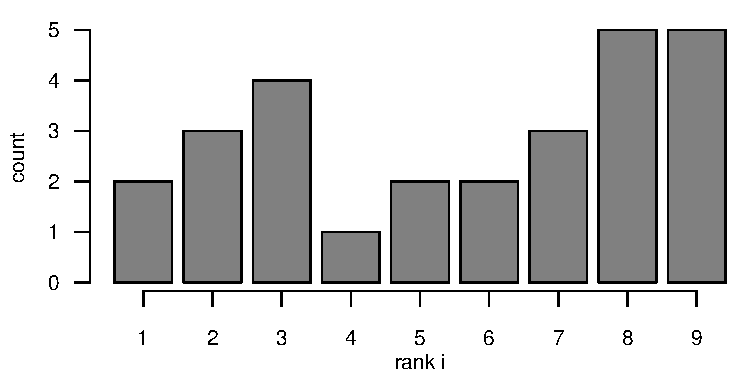
\includegraphics{fig-rank-hist}
%
\end{center}
\caption{Rank histogram}
\label{fig:rank-hist}
\end{figure}


\begin{figure}
\begin{center}
%
\begin{Hchunk}
\begin{normalsize}
\begin{Hinput}

\ttfamily\noindent
\hlprompt{{\ }}\hlfunctioncall{PlotRankhist}\hlkeyword{(}\hlsymbol{rh}\hlkeyword{,}{\ }\hlargument{mode}\hlargument{=}\hlstring{"{}prob.paper"{}}\hlkeyword{)}\mbox{}
\normalfont

\end{Hinput}


\end{normalsize}
\end{Hchunk}

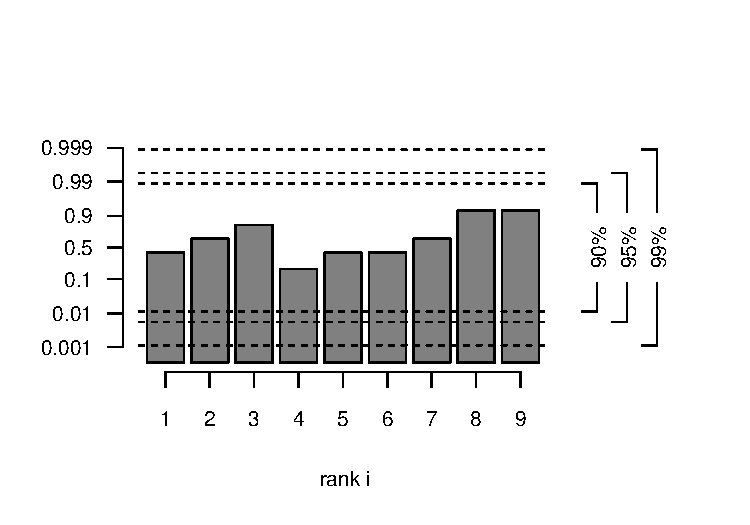
\includegraphics{fig-rank-hist-pp}
%
\end{center}
\caption{Rank histogram on probability paper}
\label{fig:rank-hist-pp}
\end{figure}


The function \code{TestRankhist} implements different statistical tests of the null-hypothesis of flat rank histogram.
Flatness of the rank histgram can be assessed by a Pearson $\chi^2$-test \citep{pearson1900criterion}.
Suppose rank $i$ was observed $r_i$ times for $i=1,\dots,R+1$, and define $e_i=N/(R+1)\ \forall\ i$ the expected number of counts if each verification rank were equally likely.
Define further
\begin{equation}
x_i = \frac{r_i - e_i}{\sqrt{e_i}}.
\end{equation}
%
Under the null-hypothesis of equally likely verification ranks, the test statistic
%
\begin{equation}
\chi^2 = \sum_{i=1}^{R+1} x_i^2
\end{equation}
%
has a $\chi^2$-distribution with $R$ degrees of freedom.


\citet{hamill2001interpretation} showed that certain types of violation of ensemble reliability are visible as different patterns in the rank histogram.
In particular, a constant bias of the mean produces sloped rank histograms, and ensembles with insufficient (excessive) ensemble spread produce $\cup$-shaped ($\cap$-shaped) rank histogram.
\citet{jolliffe2008evaluating} showed that the $\chi^2$-test statistic can be decomposed to test for sloped and convex rank histograms specifically, thus increasing the power of the test.
The test requires the definition of suitable contrast vectors $\mathbf{c}$ of length $R+1$, that satisfy $\sum_i c_i = 0$, $\sum_i c_i^2 = 1$, and $\sum_i c_i c_i' = 0$ for every pair of contrasts $\mathbf{c}$ and $\mathbf{c}'$.
Assuming a number of up to $R$ contrast vectors $\mathbf{c}^{(1)}$, $\mathbf{c}^{(2)}$, $\dots$, the test statistics $(\sum_i c^{(k)}_i x_i)^2$ are independently $\chi^2$ distributed with one d.o.f. 
The function \code{TestRankhist} uses a linear and a squared contrast. Defining $J=R+1$, the $i$-th element of the contrast vectors $\mathbf{c}^{(lin)}$ and $\mathbf{c}^{(sq)}$, for $i=1,\cdots,J$ are given by
%
\begin{align}
c^{(lin)}_i & = -\sqrt{\frac{3(J+1)}{J (J-1)}} + i \sqrt{\frac{12}{J^3 - J}}\text{, and}\\
c^{(sq)}_i & =  - \frac{\sqrt{5}  J^2 - \sqrt{5}}{\sqrt{4(J - 2)  (J-1) J (J+1) (J+2)}}+ \left(i - \frac{J+1}{2}\right)^2   \sqrt{\frac{180}{ J^5 - 5 J^3 + 4 J}}.
\end{align}
%
The $\chi^2$ test using the linear contrast is sensitive to sloped rank histgrams, i.e. biased ensembles, while the $\chi^2$ based on the squared contrast is sensitive to convex rank histograms, i.e. over- or under-dispersed ensembles.
\code{TestRankhist} returns the test-statistics and one-sided p-values of the Pearson $\chi^2$ test, and of the two tests based on the contrasts $\mathbf{c}^{(lin)}$ and $\mathbf{c}^{(sq)}$:

\begin{Hchunk}
\begin{normalsize}
\begin{Hinput}

\ttfamily\noindent
\hlprompt{{\ }}\hlfunctioncall{TestRankhist}\hlkeyword{(}\hlsymbol{rh}\hlkeyword{)}\mbox{}
\normalfont

\end{Hinput}

\begin{Houtput}

\ttfamily\noindent
{\ }{\ }{\ }{\ }{\ }{\ }{\ }{\ }{\ }{\ }{\ }{\ }{\ }{\ }{\ }pearson.chi2{\ }jp.slope{\ }jp.convex\hspace*{\fill}\\
\hlstd{}test.statistic{\ }{\ }{\ }{\ }{\ }{\ }{\ }5.3333{\ }{\ }{\ }1.6056{\ }{\ }{\ }{\ }1.3258\hspace*{\fill}\\
\hlstd{}p.value{\ }{\ }{\ }{\ }{\ }{\ }{\ }{\ }{\ }{\ }{\ }{\ }{\ }{\ }0.7214{\ }{\ }{\ }0.2051{\ }{\ }{\ }{\ }0.2496\hspace*{\fill}\hlstd{}\mbox{}
\normalfont

\end{Houtput}

\end{normalsize}
\end{Hchunk}


The rank histogram of the temperature ensemble forecast provides no evidence against the null-hypothesis of a reliable ensemble.

\section{Reliability diagrams for probability forecasts}

The reliability diagram is a classical tool to compare probability forecasts of binary events to the verifying binary observations \citep{jolliffe2012forecast}.
The reliability diagram compares the forecast probability to the conditional frequency of the observation, given the forecast.
A forecast is reliable if the forecast probability and conditional event frequency coincide.
Forecast reliability is a reasonable criterion that probability forecasts should satisfy; over all instances that the forecast issued a probability $p$, the event should happen $p\times 100\%$ of the time.

If the forecast issues probabilities that take any value on the unit interval, most forecast probabilities will be issued only once.
To estimate the conditional event frequency in this case the forecasts can be grouped into a finite number of non-overlapping bins.
The average event frequency taken over all instances where the forecast is in a given bin is then taken as an average of the conditional event frequency.
The reliability diagram is a plot of the conditional event frequency over the in-bin average of the forecast probabilities.
\pkg{SpecsVerification} provides the function \code{ReliabilityDiagram} that takes as inputs a collection of probability foredcasts and binary verifying observations, and calculates the reliability diagram for a specified number of equidistant bins, or a user-defined non-equidistant binning.
The consistency resampling method proposed by \citet{broecker2007increasing} is used to estimate the likely spread of the reliability diagrams around the diagonal if the given forecast were, in fact, reliable.


If the \code{plot} argument is set to \code{FALSE}, the \code{ReliabilityDiagram} function returns the quantities necessary to plot the reliability diagram.

\begin{Hchunk}
\begin{normalsize}
\begin{Hinput}

\ttfamily\noindent
\hlprompt{{\ }}\hlsymbol{p.bin}{\ }\hlassignement{\usebox{\hlnormalsizeboxlessthan}-}{\ }\hlfunctioncall{rowMeans}\hlkeyword{(}\hlsymbol{ens.bin}\hlkeyword{)}\mbox{}
\normalfont

\end{Hinput}


\begin{Hinput}

\ttfamily\noindent
\hlprompt{{\ }}\hlfunctioncall{ReliabilityDiagram}\hlkeyword{(}\hlsymbol{p.bin}\hlkeyword{,}{\ }\hlsymbol{obs.bin}\hlkeyword{,}{\ }\hlargument{plot}\hlargument{=}\hlnumber{FALSE}\hlkeyword{,}{\ }\hlargument{bins}\hlargument{=}\hlnumber{3}\hlkeyword{)}\mbox{}
\normalfont

\end{Hinput}

\begin{Houtput}

\ttfamily\noindent
{\ }{\ }p.avgs{\ }cond.probs{\ }cbar.lo{\ }cbar.hi{\ }p.counts{\ }bin.lower{\ }bin.upper\hspace*{\fill}\\
\hlstd{}1{\ }0.1000{\ }{\ }{\ }{\ }{\ }0.2000{\ }{\ }0.0000{\ }{\ }0.3000{\ }{\ }{\ }{\ }{\ }{\ }{\ }10{\ }{\ }{\ }{\ }0.0000{\ }{\ }{\ }{\ }0.3333\hspace*{\fill}\\
\hlstd{}2{\ }0.5227{\ }{\ }{\ }{\ }{\ }0.7273{\ }{\ }0.2222{\ }{\ }0.8333{\ }{\ }{\ }{\ }{\ }{\ }{\ }11{\ }{\ }{\ }{\ }0.3333{\ }{\ }{\ }{\ }0.6667\hspace*{\fill}\\
\hlstd{}3{\ }0.8542{\ }{\ }{\ }{\ }{\ }1.0000{\ }{\ }0.5000{\ }{\ }1.0000{\ }{\ }{\ }{\ }{\ }{\ }{\ }{\ }6{\ }{\ }{\ }{\ }0.6667{\ }{\ }{\ }{\ }1.0000\hspace*{\fill}\hlstd{}\mbox{}
\normalfont

\end{Houtput}

\end{normalsize}
\end{Hchunk}


If the argument \code{plot=TRUE} the reliability diagram is plotted, as shown in Figure \ref{reldiag-plot}. 
The logical argument \code{plot.refin} controls the refinement diagram, i.e. the histogram over the forecast probabilities.
The logical argument \code{attributes} controls plotting of the polygon defined by the vertical no-resolution line at $\bar{y} = 1/n \sum_t y_t$, where $y_t$ is the binary observation at time $t$, and the no-skill line defined by the linear equation $f(x)=(x+\bar{y})/2$, to produce the attributes diagram \citep{hsu1986attributes}.
Points that fall into the shaded area of the attributes diagram contribute positively to forecast skill defined by the Brier skill score.

\begin{figure}
\begin{center}
%
\begin{Hchunk}
\begin{normalsize}
\begin{Hinput}

\ttfamily\noindent
\hlprompt{{\ }}\hlsymbol{rd}{\ }\hlassignement{\usebox{\hlnormalsizeboxlessthan}-}{\ }\hlfunctioncall{ReliabilityDiagram}\hlkeyword{(}\hlsymbol{p.bin}\hlkeyword{,}{\ }\hlsymbol{obs.bin}\hlkeyword{,}{\ }\hlargument{plot}\hlargument{=}\hlnumber{TRUE}\hlkeyword{,}{\ }\hlargument{bins}\hlargument{=}\hlnumber{3}\hlkeyword{,}{\ }\hlargument{attributes}\hlargument{=}\hlnumber{TRUE}\hlkeyword{)}\mbox{}
\normalfont

\end{Hinput}


\end{normalsize}
\end{Hchunk}

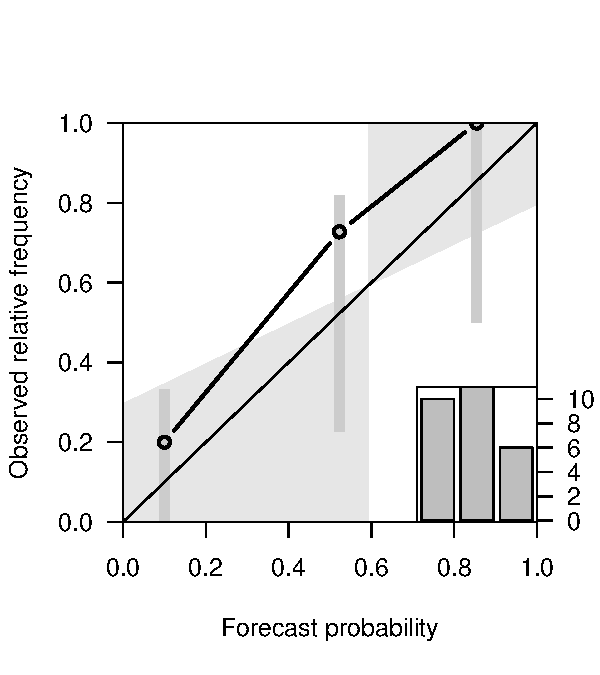
\includegraphics{fig-reldiag}
%
\end{center}
\caption{Reliability diagram}
\label{reldiag-plot}
\end{figure}


\section{Additional functions}

The focus of \pkg{SpecsVerification}, and of the present paper, is on verification functions for ensemble and probability forecasts, uncertainty quantification, and graphical display.
\pkg{SpecsVerification} includes a number of additional functions for recalibration and verification of forecasts.
For verification of deterministic forecasts, e.g. the ensemble mean forecast, the sqared error (function \code{SqErr}) and the Absolute Error (function \code{AbsErr}) have been implemented.





\section{Conclusion}

\section*{Acknowledgments}


\bibliography{ensemble-verification}

\end{document}
